\documentclass[a4paper,11pt]{article}
\usepackage[english]{babel}
\usepackage[utf8]{inputenc}
\usepackage[T1]{fontenc}
\usepackage{graphicx}
\usepackage{amsmath}
\usepackage{tikz}
\usepackage{amsthm}
\usepackage{amssymb}
\usepackage{nicefrac}
\usepackage{tabularx}
\usepackage{cprotect}
\usepackage{wrapfig}
\usepackage{framed}
\usepackage{fancyvrb}
\usepackage{bm}
\usepackage{listings}
\usepackage{longtable}
\usepackage[left=25mm,right=25mm,bottom=25mm,top=25mm]{geometry} %left, right, bottom ,top, includeheadfoot
\usepackage{caption}
\usepackage{multicol}
\usepackage{subcaption}
\usepackage{nameref}
\usepackage{placeins} %Put command \floatbarrier in front of textpassage or other items, in front of which the desired content (i.e. images) shall be placed.
\usepackage[inline]{enumitem}
% \usepackage[parfill]{parskip}
%\usepackage{fancyhdr}
\usepackage{enumitem}
\usepackage{siunitx}
\newcounter{question}
\setcounter{question}{0}
\usepackage{blindtext}
\usepackage{hyperref} %To make document linked within.
\usepackage{cleveref}
\numberwithin{equation}{section}
\captionsetup{font=footnotesize,labelfont=bf}

\renewcommand{\theenumi}{(\arabic{enumi})}
\renewcommand\labelenumi{\theenumi} % Change enumerate style from 1. to (1) etc.
\renewcommand{\theenumiii}{(\arabic{enumiii})}
\renewcommand\labelenumiii{\theenumiii} % Change enumerate style from 1. to (1) etc.
\setlist{itemsep = 0.2pt}


\newcommand\matr[1]{\ensuremath{\boldsymbol{\mathbf{#1}}}}
\newcommand\vect[1]{\ensuremath{\bm{#1}}}
\newcommand\dint{\ensuremath{\int\displaylimits}}

%\DeclareSIUnit \parsec {pc}
%\DeclareSIUnit \magnitudes {mag}
\DeclareSIUnit \curie {Ci}

\title{Deep Learning\\ \vspace{0.2cm}\normalsize Questions and Answers}
\author{Daniel Zahnd}
\date{\today}


\newtheorem{ass}{Assertion}

\begin{document}


\newcommand\Que[1]{%
   \leavevmode\par
   \stepcounter{question}
   \noindent
   \thequestion. \textbf{Q} --- #1\par}

\newcommand\Ans[2][]{%
    \leavevmode\par\noindent
   {\leftskip0pt
    \textbf{A} --- \textbf{#1}#2\par}}

\maketitle
%\thispagestyle{empty}
\tableofcontents
%\newpage

\pagenumbering{arabic}
\setcounter{page}{1}


\section{Preliminaries}
Usually, one deals with datasets containing of data $x \in \mathbb{R}^n$ associated to other data $y$ with $n \in \mathbb{N}$. The data $x$ can be scalar of vectorial, whereas the data $y$ can also be a scalar or vector. The data $x$ is either $y \in \mathbb{R}^q$ with $q \in \mathbb{R}$ or a number of a class $\{1,\dots,K\}$ for $K \in \mathbb{N}$. In the case where e.g. $y \in \mathbb{R}$, one speaks of a regression problem, whereas in the case where $y \in\{1,\dots,K\}$ are classes, one speaks of a classification task.

Usually, one has a dataset containing of various pairs of $x$ and $y$; to distinguish an instance of data from components of a vector, one writes $(x^{(i)}, y^{(i)})$ for an instance of a dataset containing of $m \in \mathbb{N}$ instances of data. For components of an instance of data $x^{(i)} \in \mathbb{R}^n$, one writes \begin{equation}
	x^{(i)} = \begin{pmatrix}
		x^{(i)}_1 \\ \vdots \\ x^{(i)}_n
	\end{pmatrix} \in \mathbb{R}^n.
\end{equation} For a whole dataset, one can write \begin{equation}
	\{(x^{(i)}, y^{(i)})\}_{i=1,\dots,m} = \{(x^{(1)}, y^{(1)}), \dots , (x^{(m)}, y^{(m)})\}.
\end{equation}

The goal in machine learning is thus to find a function $h$ with associated tunable parameters $\theta$, that predicts $y$ based on $x$; hence one can write \begin{equation}
	h_\theta(x) = y.
\end{equation} The ultimate goal usually is to determine the parameters (weights) $\theta$; whereas for the shape or nature of the function $h$, one can usually make assumptions. The $h$ is reminiscent of ``hypothesis'' and thus of ``hypothesis'' function.

\subsection{Probability measures}
\subsubsection{Random variable}
A random variable is some quantity $x$, which can take a random value. Those random values follow a certain probability distribution, which is determined by the underlying process constituting the random variable.If the probability distribution of a random variable is known, the probability density $p(x)$ can be written down for the continuous and discrete cases as \begin{equation}
	\int_{-\infty}^{\infty}p(x)\,\mathrm{d}x = 1 \qquad \text{and} \qquad \sum_{i} p(x_i) = 1.
\end{equation}

\subsubsection{Expectation value}
The expectation value $\mathbb{E}(x) \doteq \bar{x}$ of a random variable $x$ for both the continuous and discrete case is defined as \begin{equation}
	\mathbb{E}(x) = \int_{-\infty}^{\infty}xp(x)\,\mathrm{d}x \qquad \text{and} \qquad \mathbb{E}(x) = \sum_{i}x_ip(x_i).
\end{equation}

\subsubsection{Variance, standard deviation and covariance}
The variance $\mathbb{V}(x)$ of a continuous or discrete random variable $x$ can be calculated by means of \begin{equation}
	\mathbb{V}(x) = \int_{-\infty}^{\infty} (x-\bar{x})^2p(x)\,\mathrm{d}x \qquad \text{and} \qquad \mathbb{V}(x) = \sum_{i} (x_i-\bar{x})^2p(x_i).
\end{equation}
Note, that the variance $\mathbb{V}(x)$ can also be expressed as \begin{equation}\mathbb{V}(x) = \mathbb{E}\left[(x-\mathbb{E}[x])^2\right].\end{equation} The standard deviation $\sigma_x$ is defined as the square root of the variance, hence \begin{equation}
	\sigma_x = \sqrt{\mathbb{V}(x)}.
\end{equation}
Let now $x_1,\dots,x_n$ be random variables with associated probability densities $p(x_j)$, $j\in \{1,\dots,n\}$ and joint probability densities $p(x_i,x_j)$. Let furthermore be $\bar{x}_i = \mathbb{E}(x_i)$. The covariance $\mathbb{K}(x_i,x_j)$ of two random variables for the continuous and discrete case is defined as \begin{equation}\label{eq:covariance}
	\mathbb{K}(x_i,x_j) = \int_{-\infty}^{\infty}\int_{-\infty}^{\infty}(x_i-\bar{x}_i)(x_j-\bar{x}_j)p(x_i,x_j)\,\mathrm{d}x_i\,\mathrm{d}x_j
\end{equation} and \begin{equation}
	\mathbb{K}(x_i,x_j) = \sum_{k,l}(x_{i_k}-\bar{x}_i)(x_{j_l}-\bar{x}_j)p(x_{i_k},x_{j_l}).
\end{equation} Note, that the covariance $\mathbb{K}(x,y)$ of two random variables $x$ and $y$ can also be expressed as \begin{equation}\mathbb{K}(x,y) = \mathbb{E}\left[(x-\mathbb{E}[x])(y-\mathbb{E}[y])\right].\end{equation} In the context of covariance, one usually also defines the correlation coefficient $\rho(x_i,x_j)$ between two random variables as \begin{equation}\label{eq:correlationcoefficient}
	\rho(x_i,x_j) = \frac{\mathbb{K}(x_i,x_j)}{\sqrt{\mathbb{V}(x_i)\mathbb{V}(x_j)}} = \frac{\mathbb{K}(x_i,x_j)}{\sigma_{x_i}\sigma_{x_j}}.
\end{equation} % Definitions of expectation values and so on, and of Gaussian, Binomial, Poisson and Bernoulli distributions and why and when they are used

\subsection{Preliminary questions}
\Que{How is the uniform distribution defined?}
\Ans{
	Consider a continuous random variable $x$. The uniform probability distribution is defined by the probability density $p(x)$ as \begin{equation}
		p(x) = \mathcal{U}(x; a,b) = \begin{cases}
			\frac{1}{b-a} &, a \leq x \leq b \\
			0 &, \text{otherwise}
		\end{cases}
	\end{equation} where $a$ and $b$ define the domain of the distribution. The expectation value and the variance of the uniform distribution are given by \begin{equation}
		\mathbb{E}(x) = \frac{a+b}{2}, \quad \mathbb{V}(x) = \frac{1}{12}(b-a)^2.
	\end{equation} 
	
	The uniform distribution is used for processes with no prior knowledge about the probabilities of events. It is furthermore used to model processes, where all outcomes are equally likely to happen.
}

\Que{How is the standard normal distribution defined?}
\Ans{
	Consider a continuous random variable $x$. The standard normal probability distribution (Gaussian) is defined by the probability density $p(x)$ as \begin{equation}
		p(x) = \mathcal{N}(x;\mu,\sigma) = \frac{1}{\sqrt{2\pi}\sigma}e^{-\frac{(x-\mu)^2}{2\sigma^2}}
	\end{equation} where $\mu$ defines the expectation value and $\sigma$ the variance the distribution. The expectation value and the variance of the uniform distribution are given by \begin{equation}
		\mathbb{E}(x) = \mu, \quad \mathbb{V}(x) = \sigma^2.
	\end{equation} 
	
	The normal distribution is used for processes, which are influenced by an additive effect of a large number of different and independent influences modelled by arbitrary probability distributions. It pertains - with the uniform distribution - to the two default probability distributions to use, where little prior information about the modelled processes is available.
}

\Que{How is the Bernoulli distribution defined?}
\Ans{
	Consider a discrete random variable $x$. The Bernoulli probability distribution is defined by the probability density $p(x)$ as
	\begin{equation}
		p(x) = \mathcal{B}(x; p) =
		\begin{cases}
			p &, x = 1 \\
			1 - p &, x = 0 
		\end{cases},
	\end{equation}
	where $0 \leq p \leq 1$ is the probability of success (i.e., $x = 1$). The random variable $x$ takes on only two possible values: 1 (success) or 0 (failure).
	
	The expectation value and variance of the Bernoulli distribution are given by
	\begin{equation}
		\mathbb{E}(x) = p, \quad \mathbb{V}(x) = p(1 - p).
	\end{equation}
	
	The Bernoulli distribution models a single trial of an experiment where there are exactly two possible outcomes: success with probability $p$ and failure with probability $1 - p$. It is a fundamental building block of the binomial distribution, which models a sequence of independent Bernoulli trials.
}

\Que{How is the binomial distribution defined?}
\Ans{
	Consider a discrete random variable $x$. The binomial probability distribution is defined by the probability density $p(x)$ as \begin{equation}
		p(x) = \mathcal{B}(x;n,p) = \begin{cases}
			\binom{n}{x}p^x(1-p)^{n-x} &, x \in \{1,\dots,n\} \\
			0 &, \text{otherwise}
		\end{cases},
	\end{equation} where $n$ denotes the number of trials of an experiment and $p$ is the respective probability of success or failure of the outcome. The expectation value and the variance of the binomial distribution are given by \begin{equation}
		\mathbb{E}(x) = np, \quad \mathbb{V}(x) = np(1-p).
	\end{equation} 
	
	The binomial distribution is used to model processes that model a series of identical and independent experiments with exactly two possible outcomes, success or failure.
}

\Que{How is the Poisson distribution defined?}
\Ans{
	Consider a discrete random variable $x$. The Poisson probability distribution is defined by the probability density $p(x)$ as \begin{equation}
		p(x) = \mathcal{P}(x;\lambda) = \begin{cases}
			\frac{\lambda^x}{x!}e^{-\lambda} &, x \in \mathbb{N}_0 \\
			0 &, \text{otherwise}
		\end{cases},
	\end{equation} where $\lambda > 0$ defines both the expectation value and the variance. The expectation value and the variance of the Poisson distribution are given by \begin{equation}
		\mathbb{E}(x) = \lambda, \quad \mathbb{V}(x) = \lambda.
	\end{equation} 
	
	The Poisson distribution is - similarly to the binomial distribution - used to model processes that model a series of identical and independent experiments with exactly two possible outcomes, success or failure, but where the probability $p$ of success behaves as $p \rightarrow 0$ and where the number of trials $n$ behaves as $n\rightarrow \infty$.
}

\Que{How is the Poisson distribution defined?}
\Ans{
	Consider a discrete random variable $x$. The Poisson probability distribution is defined by the probability density $p(x)$ as \begin{equation}
		p(x) = \mathcal{P}(x;\lambda) = \begin{cases}
			\frac{\lambda^x}{x!}e^{-\lambda} &, x \in \mathbb{N}_0 \\
			0 &, \text{otherwise}
		\end{cases},
	\end{equation} where $\lambda > 0$ defines both the expectation value and the variance. The expectation value and the variance of the Poisson distribution are given by \begin{equation}
		\mathbb{E}(x) = \lambda, \quad \mathbb{V}(x) = \lambda.
	\end{equation} 
	
	The Poisson distribution is - similarly to the binomial distribution - used to model processes that model a series of identical and independent experiments with exactly two possible outcomes, success or failure, but where the probability $p$ of success behaves as $p \rightarrow 0$ and where the number of trials $n$ behaves as $n\rightarrow \infty$.
}

\Que{What is the popular definition of machine learning authored by Arthur Samuel in 1959?}
\Ans{According to Samuel, machine learning is the field of study that gives computers the ability to learn without being explicitly programmed. Explicitly programmed here means, that everything would be hard-coded, instead of rule-based programming.}

\Que{What is another popular definition of machine learning authored by Tom Michel in 1999?}
\Ans{
	According to Michel, a well-posed machine learning problem may be described as follows: A computer program is said to learn from experience $E$ with respect to some tasks $T$ and performance measure $P$, if its performance at tasks $T$ as measured by performance $P$ improves with experience $E$.
}

\Que{Broadly speaking, which three types of machine learning algorithms are there?}
\Ans{Broadly speaking, there are three different categories of machine learning algorithms:
	\begin{enumerate}
		\item Supervised learning: A machine learns how to make predictions about a specific target of interest, given some observations.
		\item Unsupervised learning: A machine learns how to find useful structures and patterns in given data by itself.
		\item Reinforcement learning: A machine has the ability to act and thus influence its own observations, thereby learning to make predictions to achieve a given goal.
	\end{enumerate}
	
	An example of supervised learning would be a classification task; that is to say to assign data to two or more given classes of objects depending on one or more variables. One could for example do this by means of linear or polynomial regression.
	
	In comparison to supervised learning, unsupervised learning would for example try to separate data into two or more classes of objects, depending on what makes sense to the algorithm.
	
	Reinforcement learning finally is about problems, where a sequence of decisions over time is required, where the basic idea is to implement a reward function as supervision to give the model a way to improve itself.
}

\Que{How does gradient descent work; and what is the difference between stochastic gradient descent and just gradient descent?}
\Ans{
	Gradient descent is one of the most useful and foundational techniques in machine learning; basically, it is about minimizing a loss function $J(\theta)$ with respect to weights (parameters) $\theta$ which belong to the chosen model.
	
	Hence, let now $J(\theta)$ be the loss function of a model, where $\theta = (\theta_1, \dots, \theta_n)^\top$ are the parameters of the model, which need to be optimized. The loss function might take a form as given in \cref{fig:gradientdescent}.
	\begin{figure}[h]
		\centering
		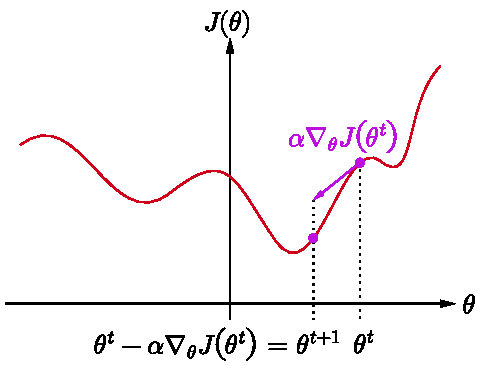
\includegraphics[width=0.4\textwidth]{figures/gradientdescent.pdf}
		\caption{Visualization of the gradient descent routine. Note, that $\theta$ is generally a vector; thus, the figure does only represent the general case in the case where $\theta$ is a scalar. If $\theta$ would consist of two components, the figure would be still visualizable in two dimensions on paper, but for higher dimensions in $\theta$, gradient descent may not be visualizable anymore on paper.}
		\label{fig:gradientdescent}
	\end{figure}
	Now, $\theta^t$ denotes the weights at iteration step $t \in \{1,\dots,T\}$ for a total iteration time $T$. Well, gradient descent updates the weights as \begin{equation}
		\theta^{t+1} = \theta^t - \alpha\nabla_\theta J(\theta^t),
	\end{equation} where the gradient is taken with respect to the weights $\theta$ and is evaluated at $\theta^t$, i.e. \begin{equation}
		\nabla_\theta = \sum_{j=1}^n e_j\partial_{\theta_j}.  \end{equation} In the case, where no confusion arises to which respect a gradient is taken, the subscript can also be left away. The parameter $\alpha$ is called the learning rate in machine learning and it has to be chosen such, that the algorithm does find the global, instead of just a local minimum of $J(\theta)$.
		
		The difference between stochastic gradient descent and just gradient descent is subtle. Stochastic gradient descent is commonly also known as minibatch gradient descent and it is computed on a small subset of all training examples, which are chose in a stochastic manner. Gradient descent is also known as batch gradient descent and is computed on the whole dataset, which takes much more time and is less efficient.
}

\Que{What is the rationale for the learning rate $\alpha$ in gradient descent?}
\Ans{
	Consider \cref{fig:gradientdescentrationale}; it shows a curve $J(\theta)$ and a quadratic function $g(\theta) = \|\theta- \theta^t\|$. Now, one can Taylor expand the function $J(\theta)$ around
	\begin{figure}[h]
		\centering
		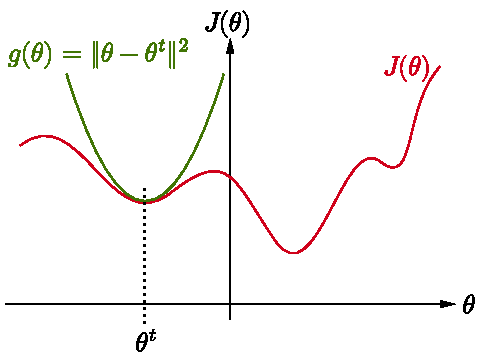
\includegraphics[width=0.4\textwidth]{figures/gradientdescentrationale.pdf}
		\caption{Rationale behind the gradient descent routine and the learning rate $\alpha$.}
		\label{fig:gradientdescentrationale}
	\end{figure} % Lecture 3 about 55min in
	an iteration step $\theta^t$ quite easily to first order in $\theta$ as \begin{equation}
		J(\theta) \approx J(\theta^t) + \nabla_\theta J(\theta^t)^\top (\theta - \theta^t).
	\end{equation} Now, the second order term would involve the Hessian, which can be quite complicated. However, one can always add a quadratic term of the form $g(\theta)$, which is scaled by some parameter $\varepsilon$, such that the resulting approximation of $J(\theta)$ always stays above the exact function; the added term with $\varepsilon$ thus approximates the Hessian. One hence has \begin{equation}
		J(\theta) \approx J(\theta^t) + \nabla_\theta J(\theta^t)^\top (\theta - \theta^t) + \frac{1}{2\varepsilon}\|\theta - \theta^t\|^2.
	\end{equation} In order to find a minimum of this expression, one has to compute the gradient of the expression with respect to $\theta$, set it to zero and solve for $\theta$. From this, \begin{equation}
		\nabla_\theta J(\theta) \approx 0 + \nabla_\theta J(\theta^t) + \frac{1}{\varepsilon}(\theta- \theta^t) \overset{!}{=} 0 \quad \Leftrightarrow \quad \theta = \theta^t - \varepsilon\nabla_\theta J(\theta^t)
	\end{equation} follows. This is nothing but gradient descent, where $\varepsilon = \alpha$ is the learning rate. As one can see, the width $(2\varepsilon)^{-1}$ of the added quadratic term to the first order Taylor expansion of $J(\theta)$ is the inverse of the learning rate. If the learning rate is large, the width of the added quadratic term is very narrow.
}

\Que{What are the main architectures used in deep learning and why are these established?}
\Ans{
	The most common architectures used in deep learning are convolutional neural networks and transformers. They are heavily used because they have proven to be useful for a wide range of problems. Oftentimes, it is not at all clear which architecture of deep learning model to use for a particular problem; but the two mentioned ones have proven to be the go-to choice at least as a first approach.
}

\Que{What is the difference between machine learning and deep learning? In what way does deep learning understand the world?}
\Ans{
The main difference between machine learning and deep learning is that machine learning describes a broader field of techniques for teaching computers to learn patterns from data, whereas deep learning refers to a subset of machine learning techniques. 

Machine learning requires feature engineering; that is, human experts need to select and potentially preprocess important features in the data. A feature in machine learning is an individual measurable property or characteristic that helps a model make predictions.

On the other hand, deep learning does not require feature engineering, as the deep neural networks learn the features from the data. This works in a sequential way; each layer in a deep neural network can be thought of learning one feature. For example, with reference to a model taking an image as an input and deciding whether it depicts a person, a car or an animal see \cref{fig:ml_vs_dl}), a first layer can be thought of detecting edges, a second is responsible for corners and contours and so on. If $x$ represents the data, a feature $\phi(x)$ is a function of the data and represents some characteristic of the data. Each layer in a deep neural network can be thought of as a $\phi_j(x)$, that is as a function that extracts one feature from the data. The model then makes its prediction $f(x)$ in the end based on a concatenation of each $\phi_j(x)$, that is $f(x) = g(\phi_n \circ \dots \circ \phi_1(x))$, where $g(x)$ represents some function of the individual features.
\begin{figure}[h]
	\centering
	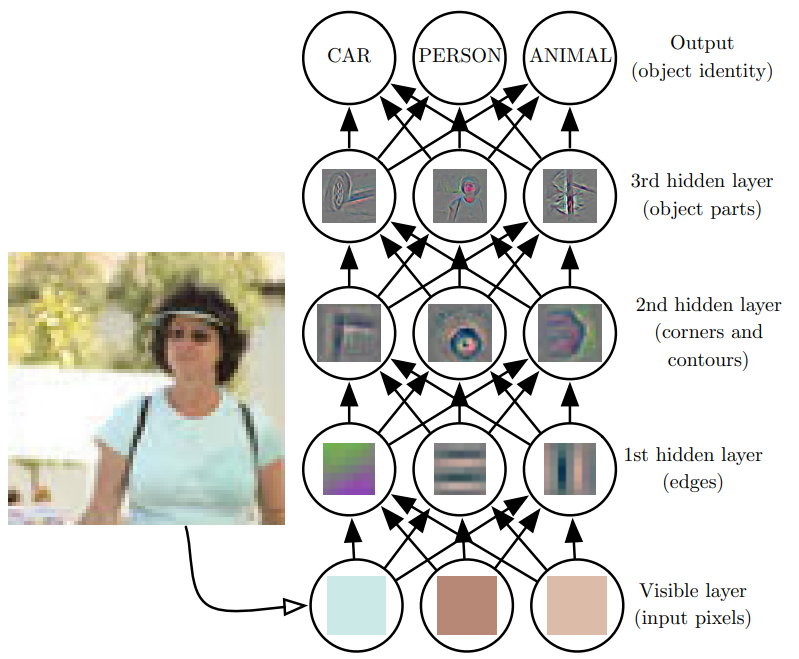
\includegraphics[width=0.4\textwidth]{figures/ml_vs_dl.png}
	\caption{Working principle of a deep neural network.}
	\label{fig:ml_vs_dl}
\end{figure}
 % Lecture 1 slides 37ff
}

\Que{What are the main similarities between deep learning and the (human) brain? What interesting insights from neuroscience are there for deep learning?}
\Ans{
Researchers working with mice have shown, that mammal brains seem to work in a hierarchical manner. That is to say that one level of neurons is responsible for detection of low-level features such as response to light sources. Another level of neurons in hierarchical succession to the first level is then tasked with detection of higher-order features such as light source movement; even another level could be responsible for light source shape; and so on.

This parallels the structure of neural networks in deep learning. It is the case that each layer of neural networks is responsible for detection of some feature. In the end, the neural network consisting of many layers of neurons is a collaboration of each neural network layer to detect multi-featured objects.   % Hierarchical structures, each layer for one feature, Lecture 1 slides 45ff
}

\Que{Which are the parallels of better and deeper models to the cognitive abilities of living beings?}
\Ans{
It seems to be the case that the more layers and the more connections each neuron in a layer has to other neurons in other layers, the better an artificial neural network will perform a given task. This is why the study of artificial neural networks is sometimes called deep learning and why one speaks of deep neural networks - because artificial neural networks get better, the deeper they are. 
\begin{figure}[h]
	\centering
	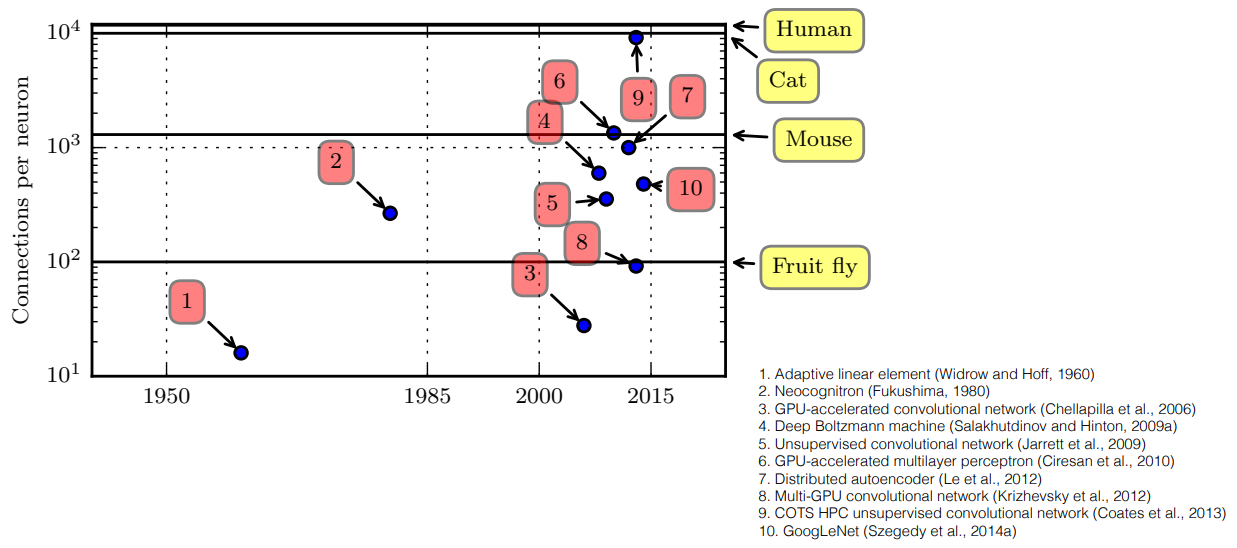
\includegraphics[width=0.8\textwidth]{figures/deepermodels.png}
	\caption{Published AI neural networks and their specification in terms of connections per neuron.}
	\label{fig:deepermodels}
\end{figure}

It is interesting, that with progressive time, deep neural networks perform better. In 2025, it is truly amazing what for example a large language model (LLM) can do! What \cref{fig:deepermodels} shows is the number of connections per neuron versus progressing time for certain published deep neural networks. Comparing the number of connections per neuron with experimental data from biology, it is evident that deep neural networks slowly but steadily approach human level in terms of connections per neuron. Looking at \cref{fig:deepermodels}, there seems to be a connection between cognitive abilities of living beings and the number of connections per neuron. % Lecture 1 slide 49ff
}

\Que{With respect to datasets and labels; why is it for example not necessary for visual tasks to have more than a several thousands of categories?}
\Ans{
Consider a dataset $\{(x^{(1)},y^{(1)}),\dots,(x^{(m)},y^{(m)})\}$ of data $x^{(j)} \in \mathbb{R}^n$ with labels $y^{(j)} \in \{1,\dots,k\}$. A visual task requires a model that associates a label $y^{(j)} \in \{1,\dots,k\}$ to each image $x^{(j)}$. Now, an image may portray some object, which one would classify by a word from a vocabulary in a certain language. In the English language, there are about half a million words of general vocabulary, and another half a million of words from the technical and scientific fields. In total, one can say that there are about a million words present in the vocabulary. Clearly, not all of these words can be visualized in a non-mistakeable way; for example ``empty'', ``transparent'' and such words. Hence, the standard vocabulary describing any set of images would likely be no longer than several thousands of words; hence, only that number of categories $k$ are commonly required in computer vision. % Slide 58ff
}

\Que{What is one-hot encoding and why is it useful?}
\Ans{
	One-hot encoding is a method for representing categorical variables as binary vectors. It is commonly used in machine learning and data preprocessing to convert non-numeric labels into a numerical form that can be processed by algorithms, which typically require numeric input. 
	
	Suppose you have a categorical feature called \texttt{Color} with three categories: \texttt{Red}, \texttt{Green}, and \texttt{Blue}. With one-hot encoding, this would be represented as follows:
	
	\[
	\begin{array}{|c|c|c|c|}
		\hline
		\text{Color} & \text{Red} & \text{Green} & \text{Blue} \\
		\hline
		\text{Red} & 1 & 0 & 0 \\
		\text{Green} & 0 & 1 & 0 \\
		\text{Blue} & 0 & 0 & 1 \\
		\hline
	\end{array}
	\]
	
	Each category gets its own binary column, and only one column is ``hot'' (i.e., set to 1) for each instance. This encoding is useful because most machine learning models cannot directly handle categorical text data, and one-hot encoding makes the data numerical and suitable for algorithms. Unlike label encoding, one-hot encoding does not assume any ordinal relationship between the categories (for example, it avoids assigning \texttt{Red = 0}, \texttt{Green = 1}, and so on, which could imply an arbitrary order). One-hot encoding generally improves model performance, especially for algorithms like logistic regression or neural networks.
	
	However, there are some considerations. If there are many unique categories, one-hot encoding can result in a large number of columns, which may increase memory usage and impact performance. Additionally, since most of the values in the one-hot encoded vectors are zero, sparse matrix representations are often used to optimize storage and processing.
}

\section{Machine learning review}
\Que{What is supervised learning? What is the goal of supervised learning?}
\Ans{
	Suppose that one has a dataset $\{(x^{(i)}, y^{(i)})\}_{i=1,\dots,m}$ of feature vector $x\in\mathbb{R}^n$ samples and associated labels $y \in\{1,\dots,K\}$. Supervised learning is about learning the parameters $\theta$ for a model that models a probability density $p(y|x; \theta)$. % Lecture 9
}

\Que{What is unsupervised learning? What is the goal of unsupervised learning?}
\Ans{
	Suppose that one has a dataset $\{x^{(i)}\}_{i=1,\dots,m}$ of feature vector $x\in\mathbb{R}^n$ samples. Unsupervised learning is about learning the parameters $\theta$ of a model that models a probability density $p(x; \theta)$. % Lecture 9
}

\Que{What is the principle of reinforcement learning?}
\Ans{
	Reinforcement learning (RL) is a framework for learning how to make sequential decisions by interacting with an environment. Unlike supervised learning, where the correct labels are provided for each input, RL provides feedback in the form of a reward signal. The principle of RL is to learn a policy that maps states to actions in order to maximize the cumulative reward over time. 
	
	For example, in a robot walking task, the robot receives positive rewards for moving forward and negative rewards for falling over. The RL algorithm's goal is to learn an action strategy that maximizes the total accumulated rewards. By trial and error, and using the reward signal as feedback, the learning agent discovers the actions that lead to desirable outcomes.
}

\Que{Which are three often used assumptions in machine learning?}
\Ans{The three main assumptions are: \begin{enumerate}
		\item Feature data $x$ and associated data $y$ (related by a model $y=f(x;\theta)$) are modeled by means of a parametric probability density, that is to say, one assumes, that the data follows a probability density \begin{equation}
			p = p(y|x;\theta),
		\end{equation} where $\theta$ are the model parameters.
		\item The data is assumed to be independent and identically distributed (IID). This assumption allows to write a joint probability distribution $p(y^{(i)},\dots,y^{(m)}|x^{(1)},\dots,x^{(m)};\theta)$ as a simple product, namely \begin{equation}
			p(y^{(i)},\dots,y^{(m)}|x^{(1)},\dots,x^{(m)};\theta) = \prod_{i=1}^m p(y^{(i)}|x^{(i)};\theta).
		\end{equation}
		\item The maximum likelihood approach can be used to identify the model parameters $\theta$ for the model $y = f(x;\theta)$, that is to say the optimal model parameters are found by means of \begin{equation}
			\hat{\theta} = \arg\max_{\theta} \left(\sum_{i=1}^{m}\ln \left[p(y^{(i)}|x^{(i)};\theta) \right]\right).
		\end{equation}
\end{enumerate}}

\Que{How is the maximum likelihood approach for optimization problems defined in the context of supervised learning?}
\Ans{
	Suppose, that one has data $y$ associated to other data $x$ by means of a model \begin{equation}
		y \approx h_\theta(x),
	\end{equation} that depends on some model parameters $\theta$, which are to be found. What has to be assumed for the model $h_\theta(x)$ is that $y|x$ follows a certain probability density $p(y|x)$. Suppose now, that one has samples \begin{equation}
		\{(x^{(i)}, y^{(i)})\}_{i=1,\dots,m}
	\end{equation} that are independently and identically distributed, one can find the model parameters $\theta$ by means of the so-called maximum likelihood approach. One calculates \begin{align}
		\begin{aligned}
			p(y^{(1)},\dots,y^{(m)}|x^{(1)},\dots,x^{(m)};\theta) = \prod_{i=1}^m p(y^{(i)}|x^{(i)};\theta).
		\end{aligned}
	\end{align} Hereby, the identically and independently distributed (IID) assumption has been used to write the joint probability as a product. Now, in order to find the model parameters $\theta$, this probability has to be maximized, since it should be highly likely to get precisely the samples $\{(x^{(i)}, y^{(i)})\}_{i=1,\dots,m}$. Therefore, the model parameters $\hat{\theta}$ are given by 
	\begin{align}
		\begin{aligned}
			\hat{\theta} = \arg\max_{\theta} \left(\sum_{i=1}^{m}\ln \left[p(y^{(i)}|x^{(i)};\theta) \right]\right).
		\end{aligned}
	\end{align} Taking the logarithm of the probability renders the product as a sum, without changing the argument of maximal probability in $\theta$.
}

\Que{What is regularization?}
\Ans{
	Regularization describes a family of approaches that ensure, that a trained model generalizes well. That is to say, regularization aims for the goal of good performance of a trained model on unseen data. 
	
	Consider for example, that one has a set $M = \{M_1,\dots,M_n\}$ of $n$ models trained on a dataset $S$. Assume, that $M_k$ is a $k$-th order polynomial model. It is known, that a higher order polynomial will better fit the training data $S$. However, one will also fit the uncertainty present in the training data $S$, which will lead to bad performance on new, unseen data. One calls this overfitting; and regularization is the means to prevent a model from overfitting during training. % Lecture 8
}

\Que{How is the Bayes risk defined and what does it mean?}
\Ans{
Suppose that one has a dataset $\{(x^{(i)}, y^{(i)})\}_{i=1,\dots,m}$ of feature vector $x\in\mathbb{R}^n$ samples and associated labels $y \in\{1,\dots,K\}$. Let furthermore \begin{equation}
	f(x^{(j)}) \approx y^{(j)}
\end{equation} be a predictor model trained on that dataset. In addition to this $\mathcal{L}(f(x^{(j)}),y^{(j)})$ shall denote a loss function accounting for the discrepancy between the prediction $f(x^{(j)})$ and the true label $y^{(j)}$. Now, the optimal predictor function $f^\star(x)$ is found by means of minimizing the so-called Bayes risk, which is defined as \begin{equation}
R(f) = \mathbb{E}_{x,y}[\mathcal{L}(f(x),y)] = \int \mathcal{L}(f(x),y)p(x,y)\,\mathrm{d}x\,\mathrm{d}y.
\end{equation} Hereby, $p(x,y)$ is the joint probability density of feature vectors and labels. Hence, we have \begin{equation}
f^\star(x) = \arg\min_f\left[R(f)\right].
\end{equation} The Bayes risk is an average loss. The joint probability density $p(x,y)$ is a weighting factor of the loss; the loss is weighted more strongly for those sample combinations $(x,y)$, which are very probable to occur in the dataset. In practical applications, one needs to specify a particular probability density $p(x,y)$ in order for the Bayes risk to be calculable.
} % Slide 15

\Que{How is the empirical risk defined and how does it relate to the Bayes risk?}
\Ans{The empirical Bayes risk $\hat{R}(f)$ is obtained from the Bayes risk definition by the specification $p(x,y)$ as a uniform distribution. This means, that the loss $\mathcal{L}(f(x^{(j)}),y^{(j)})$ is weighted equally for all sample pairs $(x^{(j)},y^{(j)})$. Furthermore, due to the discrete nature of samples, the integral in the Bayes risk definition transforms to a sum as \begin{equation}
		\hat{R}(f) = \frac{1}{m}\sum_{i=1}^m \mathcal{L}(f(x^{(i)}), y^{(j)}).
	\end{equation} The optimal predictor $\hat{f}$ as found by the empirical Bayes risk is then given by \begin{equation}
	\hat{f}(x) = \arg\min_f\left[\hat{R}(f)\right].
	\end{equation}% Slide 16
}

\Que{What are train, validation and test splits for?}
\Ans{
	Given some model $M$ and a training dataset $S = \{(x^{(i)}, y^{(i)})\}_{i=1,\dots,m}$, one usually divides the data into training and testing data as \begin{equation}
		S_{test} \subset S, \qquad S_{train} \subset S, \qquad S_{test} \cap S_{train} = \emptyset, \qquad S_{test} \cup S_{train} = S.
	\end{equation} The training set $S_{train}$ is only used to train the model $M$, while the test set $S_{test}$ is solely used to test the model after final training. There however is also such a thing as the validation set. The validation set is used to determine the optimal hyperparameters for the model $M$, such as the polynomial degree for a polynomial regression model. Oftentimes, the validation set is chosen as a subset of the training dataset (e.g. via the cross validation technique). The reason why the test dataset is not used for hyperparameter setting is that one would use information gained by the test dataset to ``improve'' the model; but that could lead to overfitting and less performance on unseen data; the test data would thus become some sort of training data.
	% Lecture 8
}

\Que{How are Bayesian statistics used for regularization?}
\Ans{
	Conceiving of the weights $\theta$ of a model not as being unknown and constant, but as being unknown and a random variable following the density $p(\theta)$, one can derive the optimal weights $\hat{\theta}$ as \begin{equation}
		\hat{\theta} = \arg\max_\theta\left(\prod_{i=1}^{m}p(y^{(i)}|x^{(i)},\theta)p(\theta)\right)
	\end{equation} using Bayesian statistics. This technique is known as maximum a posteriori estimation. Compared to the maximum likelihood estimation technique, we have an added term $p(\theta)$ here, which takes care of regularization. Due to this term, the found weights using maximum a posteriori estimation will generally have a smaller norm than those of maximum likelihood estimation and are thus less sensitive to fluctuations in new data $x^{(k)}$, $y^{(k)}$; this means, that a model trained using maximum a posteriori estimation will generalize better than a maximum likelihood trained one.
}

\section{Deep forward networks}
\subsection{Network architecture}

\Que{What is a feedforward neural network and what is the vocabulary for it?}
\Ans{
	A feedforward neural network is basically just a concatenation of many very simple functions of an input (vector) $x \in \mathbb{R}^n$; \cref{fig:ffn_struc} visualizes that. The functions of the neural network are interconnected to each other, such that it takes for example an image as input, and outputs a label $y$ at the end, e.g. ``car'' or ``horse''. There is an established, common terminology used in the context of neural networks. This terminology is visualized in \cref{fig:ffn_voc}. A feedforward neural network can have a depth and width of any choice; the only limitation is computational power and memory.
	\begin{figure}[h]
		\centering
		\begin{subfigure}{0.49\textwidth}
			\centering
			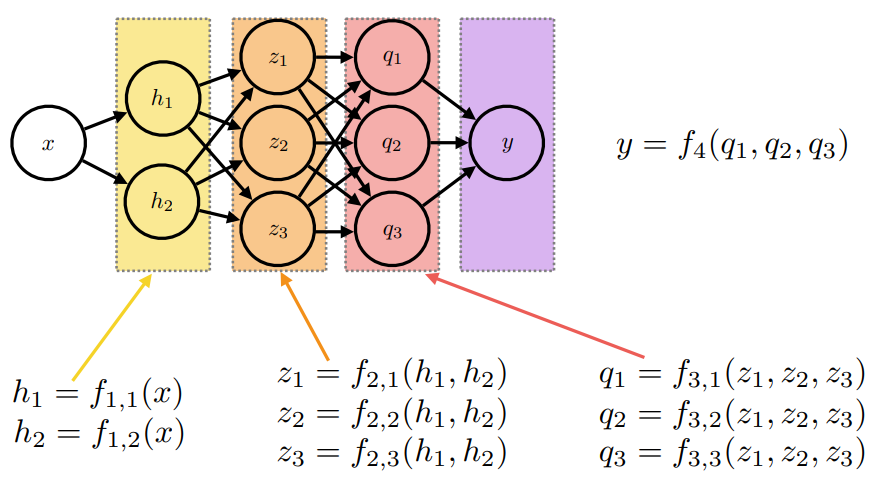
\includegraphics[width=\textwidth]{figures/ffn_struc.png}
			\caption{Structure of a feedforward neural network.}
			\label{fig:ffn_struc}
		\end{subfigure}\hfill
		\begin{subfigure}{0.49\textwidth}
			\centering
			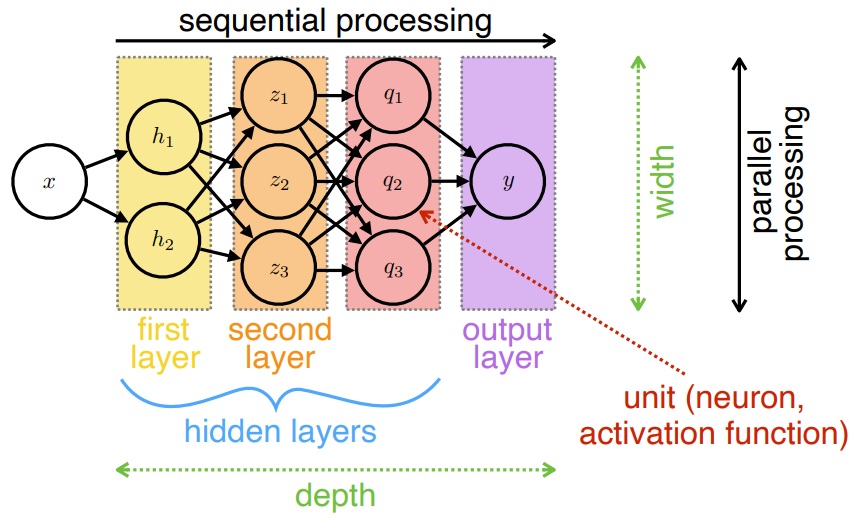
\includegraphics[width=\textwidth]{figures/ffn_voc.png}
			\caption{Vocabulary associated to feedforward neural networks.}
			\label{fig:ffn_voc}
		\end{subfigure}
		\caption{Structure and vocabulary of feedforward neural networks.}
		\label{fig:ffn}
	\end{figure}  % Lec 2-3, slide 4-5
}

\Que{What is the analogy of feedforward neural networks to the (human) brain?}
\Ans{
A feedforward neural network consists of so-called (artificial) neurons. The concept of such a neuron is inspired by its real equivalent in nature - such as that in a human brain. The analogies of an artificial neuron - also known as a perceptron - to the neuron of a (human) brain is visualized in \cref{fig:analogy}.
\begin{figure}[h]
	\centering
	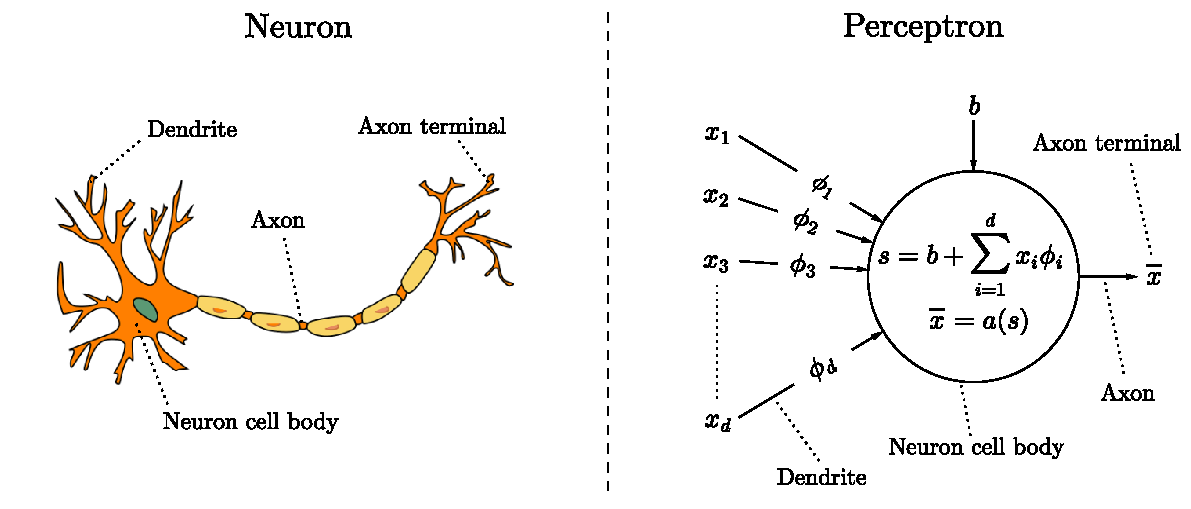
\includegraphics[width=0.6\textwidth]{figures/analogy.pdf}
	\caption{Analogy of the perceptron (artificial neuron) to its equivalent in nature.}
	\label{fig:analogy}
\end{figure} 
The perceptron consists of inputs, which are the components of an input vector $x = (x_1,\dots,x_d)^\top$. Each component $x_i$ is weighted by a weight $\phi_i$. In addition to the components, a certain bias $b$ is added. Altogether, the contributions from the components (dendrites) are summed up to a sum $s= b + \sum_{i=1}^d x_i\phi_i$. In analogy to the neuron in the (human) brain, this sum of the contributions (dendrites) needs to achieve a certain threshold to produce an output, hence a so-called activation function $a(s)$ is introduced. The output $\bar{x}$ of the perceptron is then the sum $s$ passed to the activation function, namely $\bar{x} = a(s)$.
}

\Que{What are the key aspects of any feedforward neural network?}
\Ans{
The key aspects of any feedforward neural network are visualized in \cref{fig:keyaspects}. Essentially, there is a training set of data (usually feature vectors $x^{(i)}$ and labels $y^{(i)})$) from which one can learn information. Then, there is a network model, which consists of an input layer, hidden layers and an output layer. Basically, the network model is a function $f(x^{(i)};\theta)$ parametrized with weights $\theta$, which takes an input vector $x^{(i)}$ and outputs a vector that has the same dimensionality as the label vector or scalar $y^{(i)}$. What is trained in a feedforward network are the weights $\theta$ parametrizing the function $f(x^{(i)};\theta)$. This is done by optimizing the weights $\theta$ with respect to a cost function $\mathcal{L}(y^{(i)},f(x^{(i)};\theta))$ that takes as input the ground truth $y^{(i)}$ given by the training data and the predicted label $f(x^{(i)}, \theta)$ that is given by the input $x^{(i)}$ and the network weights $\theta$. The input layer must be of dimensionality as $x^{(i)}$, whereas the output layer needs to have dimensionality of $y^{(i)}$. In between, the hidden layers can have any dimensionality of choice.
\begin{figure}[h]
	\centering
	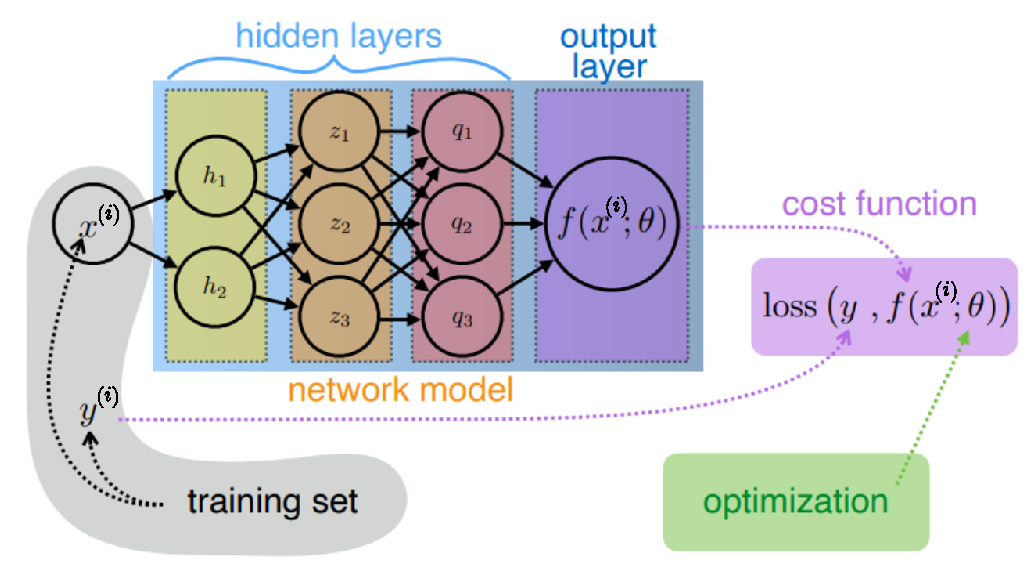
\includegraphics[width=0.5\textwidth]{figures/keyaspects.pdf}
	\caption{Key aspects of any feedforward neural network.}
	\label{fig:keyaspects}
\end{figure}
}
\Que{What is saturation in the context of gradient descent?}
\Ans{Saturation is an effect that can occur in optimization problems. Say, one has cost function $\mathcal{L}(\theta)$ to optimize. If the cost function has flat regions, the gradients are very small in those regions and therefore gradient descent to train neural networks can progress only very slowly or comes to a halt. This is what is known as saturation.

The saturation issue is commonly overcome by using cost functions (loss functions) that have non-flat regions, when the prediction is incorrect. Correct predictions are mapped to flat space, whereas incorrect predictions map to non-flat space. This ensures, that gradient descent on the loss function $\mathcal{L}(\theta)$ progresses fast, when the predictions of the trained network are far from correct and slow, when almost all predictions are correct.} % Slide 22, lec 2-3}

\Que{What are the main activation functions used commonly for output layers or hidden layers in neural networks? What are their most prominent properties?}
\Ans{The most prominent activation functions used in hidden layers to introduce nonlinearities into a function $f(x^{(i)};\theta))$ modelling the predicted labels $y^{(i)}$ are the following:
\begin{enumerate}
	\item \textbf{ReLU}: ReLU stands for rectified linear unit and mathematically, it is given by \begin{equation}
		g(z) = \max\{0,z\}.
	\end{equation} An important property of this function is that the gradients are zero for $z < 0$ and hence gradient descent cannot make any progress if an output of a neuron in a neuronal network is below zero. Furthermore, strictly speaking it it is not differentiable at $z=0$, which makes calculation of a gradient at this point impossible. However, in practice this has been shown to be irrelevant as this issue has non-significant effects. This is why ReLU is probably the top used activation function.
	\item \textbf{Softplus:} The softplus function is defined mathematically as \begin{equation}
		g(z) = \log(1+\exp(z))
	\end{equation} and hence is a- smooth approximation of ReLU, which is hence differentiable at the point $z=0$. It has therefore very similar properties to ReLU.
	\item \textbf{Hyperbolic tangent:} The hyperbolic tangent \begin{equation}
		g(z) = \tanh(z)
	\end{equation} is sometimes used as an activation function for hidden layers. It has a range from $-1$ to $1$ and is zero-centered. They are heavily used in recurrent neural networks.
	\end{enumerate}

In addition to this, the most prominent activation functions used in output layers to introduce nonlinearities into a function $f(x^{(i)};\theta))$ modelling the predicted labels $y^{(i)}$ are the following:
\begin{enumerate}
	\item \textbf{Sigmoid:} The sigmoid function defined by \begin{equation}
		g(z) = \frac{1}{1+e^{-z}}
	\end{equation} is used for binary classification tasks, because it can be nicely interpreted as giving a probability measure for $z$ to belong either to class 0 or class 1.
	\item \textbf{Softmax:} The softmax function defined by \begin{equation}
		g(z)_i = \frac{e^{z_i}}{\sum_{j=1}^k e^{z_j}}
	\end{equation} is the generalization of the sigmoid function to classification tasks with more than two classes, where $g(z)_i$ is interpreted as the probability of the original input vector $x^{(j)}$ to belong to class $i \in \{1,\dots,k\}$ belonging . This is to say that if there are two classes, the softmax function is identical to the sigmoid function.
\end{enumerate}
} % Slides 26-42, lec 2-3


\Que{How is the numerical implementation of the softmax functions realized in a numerically stable way?}
\Ans{Note, that the softmax function is defined by \begin{equation}
		g(z)_i = \frac{e^{z_i}}{\sum_{j=1}^{k}e^{z_j}}.
\end{equation} Notice, that for $z_i \ll 1$ or $z_i \gg 1$, the exponential tends to grow extremely fast. Hence, numerical stability is compromised for very small or very large values of $z_i$. The softmax function however has the property of being invariant to shifts, as \begin{align}
\begin{aligned}
	g(z-a)_i = \frac{e^{z_i - a}}{\sum_{j=1}^{k}e^{z_j-a}} = \frac{e^{-a}e^{z_i}}{e^{-a}\sum_{j=1}^{k}e^{z_j}} = g(z)_i
\end{aligned}
\end{align} for $a \in \mathbb{R}$ shows. Hence, one can calculate the maximal value contained in the vector $z$ as $\max_j(z_j)$ and subtract it from all components of $z$, i. e. \begin{equation}
g(z-\max_j[z_j])_i = g(z)_i.
\end{equation} This performs a shift operation ``normalizing'' the largest value in $z$ to 1, and all other values smaller than 1. Since it is just a shift operation, it leaves the softmax invariant, but is numerically stable, as one has no extremely large or small values to calculate the exponential for.
} % slide 30, lec 2-3 
%
%\Que{What are the main activation functions used commonly for hidden layers? What are their most prominent properties?}
%\Ans{Text.} % Slides 35ff, lec 2-3
%
%\Que{What are the main activation functions used commonly for output layers? What are their most prominent properties?}
%\Ans{Text.} % Slides 35ff, lec 2-3

\Que{What is the universal approximation theorem in network architecture?}
\Ans{The universal approximation theorem states, that a feedforward network with a linear output layer and enough - but at least one - hidden nonlinear layers can approximate any function between two finite-dimensional spaces up to any desired precision. In mathematical terms, let $N \subseteq \mathbb{R}^n$ and $M \subseteq \mathbb{R}^m$ be two finite-dimensional spaces and let \begin{equation}
		f: N \rightarrow M; \quad x \mapsto y = f(x)
	\end{equation} be a function producing samples $\{(x^{(i)}, y^{(i)})\}_{i=1,\dots,k}$. The universal approximation theorem states there exist an neural network $\tilde{f}$ parametrized by weights $\theta$ with the above requirements that can represent the function $f$ to any desired precision, i. e. $f(x) \approx \tilde{f}(x;\theta)$. It is however not guaranteed, that the network can learn this representation from the samples $\{(x^{(i)}, y^{(i)})\}_{i=1,\dots,k}$.} % Slides 44ff, lec 2-3

\Que{What type of modification to a network architecture generally improves the performance the most?}
\Ans{
	It seems to be the case that depth of a neural network (i. e. how many hidden layers) is the most influential architectural factor. The reason for this is that depth enables a neural network to break down complex tasks and representations into manageable, simple subproblems. That is, a deep neural network represents a complex function by many simple sub-units. The deeper the network, the better a neural network generalizes.} % Slide 46ff

\Que{Which are the key ingredients and insights to the training (optimization) of a model}
\Ans{
The key ingredients needed to train a neural network are the following:
\begin{itemize}
	\item The training data. In order for a neural network $\tilde{f}(x;\theta)$ to learn a representation of a data-producing function $f(x)$, there need to be training data $\{(x^{(i)}, y^{(i)})\}_{i=1,\dots,k}$.
	\item The network design. In order for a neural network to build a representation of a data-producing function, a design $\tilde{f}(x;\theta)$ parametrized by adjustable weights $\theta$ is needed.
	\item The loss function. In order to allow the network to adjust its parameters $\theta$ such that $f(x) \approx \tilde{f}(x;\theta)$, a loss function incentivizing a change in $\theta$ towards closer resemblance of $f$ with $\tilde{f}$ is required.
\end{itemize}
Iteratively changing the weights $\theta$ of a neural network towards closer resemblance of $f$ with $\tilde{f}$ is known as training or optimization.
} %  Slides 49-60, lec 2-3


\Que{What are computational graphs and how are they built? Give an example!}
\Ans{Computational graphs are directed acyclic graphs that represent the structure of a function through a sequence of operations on inputs and intermediate variables. Each node corresponds to either a variable (such as an input, parameter, or intermediate result) or an operation (such as addition or multiplication). The edges represent the flow of data between these operations. Building a computational graph involves decomposing a complex function into elementary operations, each of which is assigned a node.
	
	For example, consider the scalar function
	\begin{equation}
		J = (x \cdot w + b)^2,
	\end{equation}
	where \( x \), \( w \), and \( b \) are inputs. This function can be broken down into the following intermediate steps:
	\begin{equation}
		u_1 = x \cdot w, \quad u_2 = u_1 + b, \quad J = u_2^2.
	\end{equation}
	Each of these steps forms a node in the computational graph. This structure allows us to perform both forward and backward passes efficiently and is especially useful for computing gradients using back-propagation.
}

\Que{What is back-propagation and how does it work?}
\Ans{Back-propagation is an algorithm used to efficiently compute gradients of a scalar output (typically a loss function) with respect to the inputs or parameters of a model, by applying the chain rule of calculus through a computational graph. The process involves two phases: A forward pass and a backward pass.
	
	In the forward pass, we compute the value of each node in the graph from inputs to output. In the backward pass, we start at the output node and recursively compute gradients of the output with respect to each node by applying the chain rule. For a node \( u_j \), the gradient of the output \( J \) with respect to \( u_j \) is given by
	\begin{equation}
		\frac{\partial J}{\partial u_j} = \sum_{i: u_j \in \text{Parents}(u_i)} \frac{\partial J}{\partial u_i} \cdot \frac{\partial u_i}{\partial u_j}.
	\end{equation}
	This recursive formulation enables the reuse of intermediate gradients, which makes the computation more efficient than computing derivatives from scratch. Back-propagation is at the core of training deep neural networks using gradient-based optimization methods.
}

\Que{With respect to what and how are gradients calculated in the context of computational graphs?}
\Ans{In the context of computational graphs, gradients are calculated with respect to the leaf nodes of the graph, which typically correspond to model parameters such as weights and biases. The goal is to determine how a small change in each parameter affects the final output, usually a scalar loss function \( J \).
	
	The calculation uses the chain rule applied through the graph. Suppose the graph ends in output \( u_n \) and a parameter \( \theta_j \) is one of the inputs. Then the gradient of the output with respect to \( \theta_j \) is computed as
	\begin{equation}
		\frac{\partial J}{\partial \theta_j} = \frac{\partial u_n}{\partial u_{n-1}} \cdot \frac{\partial u_{n-1}}{\partial u_{n-2}} \cdots \frac{\partial u_k}{\partial \theta_j}.
	\end{equation}
	This product of partial derivatives reflects how a change in \( \theta_j \) propagates through the computational graph to influence the output. In practice, this is implemented via reverse-mode automatic differentiation, or back-propagation, which efficiently computes these gradients by traversing the graph backward and accumulating gradient information at each step.
}

\subsection{Regularization}
\Que{With respect to training a neural network: What is the best number of epochs to train a model?}
\Ans{
Consider some training process of a neural network as visualized in \cref{fig:best_num_epochs}. The best number of epochs is located, where the test error has a minimum. The test error is the given by one minus the test precision. As such, it is a measure of how many predictions made by the neural network are wrong on the test set. For example, if the error is 0.03, it means that 3 predictions out of 100 on the test set are wrong.
\begin{figure}[h]
	\centering
	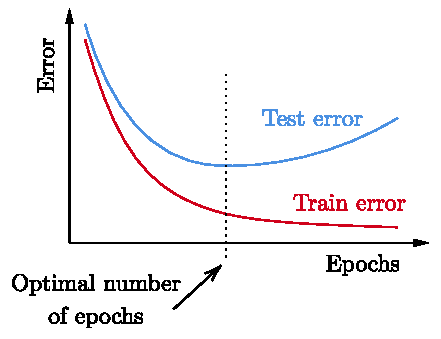
\includegraphics[width=0.35\textwidth]{figures/best_num_epochs.pdf}
	\caption{Visualization of an example case of a train and test error of a neural network.}
	\label{fig:best_num_epochs}
\end{figure}
Training of a neural network should be continues, whenever the test error is observed to descend continuously, but stopped as soon as the test error is seen to rise steadily again. The reason for this is that a rising test error - while the train error continues to go down - indicates, that the model has overfitted. It means that the model has learned to fit the training data almost perfectly, but as a result performs poorly on unseen data.
}

\Que{What is generalization in the context of neural networks and what are the main issues with it?}
\Ans{Generalization in the context of neural networks refers to the ability of those networks to effectively learn meaningful patterns from the data. Typically, there can occur two major problems when fitting or training any model to data, namely overfitting and underfitting.

Underfitting occurs, when there are too few model parameters. This results in a large bias, but low variance. Overfitting however arises, whenever there are too many model parameters. The consequence of this is that one has a small bias, but high variance. Neural networks typically have problems with overfitting, which makes the use of regularization techniques necessary in training. Regularization is a term for any kind of technique to reduce the natural tendency for overfitting in neural networks.} % Slides 4ff, Lec 4

\Que{Which are the main strategies to tackle the issue of overfitting in neural networks?}
\Ans{
	There are three main categories of techniques employed to reduce overfitting in neural network training:
	\begin{enumerate}
		\item Constrain the model: This is to say that the model family is restricted or the parameter space (measure for the amount of model parameters) is constrained with a suitable threshold.
		\item Modify loss function: This strategy is all about adding suitable terms to the loss function, which have the effect of penalizing too many model parameters.
		\item Ensembling methods: Ensembling methods means to train several different models on the same data and use a combined model to make predictions. This is known to reduce both the variance and bias of the combined model with respect to the ingredient models.
	\end{enumerate}
} % Slides 5ff, Lec 4

\Que{How does regularization using the maximum a posteriori estimate work?}
\Ans{
	Regularization using the maximum a posteriori (MAP) estimate is a Bayesian interpretation of regularization in machine learning. The idea is to regard the model parameters $\theta$ as random variables.
	
	Given data $\mathcal{D} = \{(x_i, y_i)\}_{i=1}^n$ and a model with parameters $\theta$, the goal is to find the most probable parameters $\hat{\theta}_{MAP}$ given the data, i.e.,
	\begin{equation}
		\hat{\theta}_{MAP} = \arg\max_{\theta} \left[\, p(\theta \mid \mathcal{D})\, \right].
	\end{equation} Using the Bayes theorem we get
	\begin{equation}
		p(\theta \mid \mathcal{D}) = \frac{p(\mathcal{D} \mid \theta) p(\theta)}{p(\mathcal{D})}.
	\end{equation} Since $p(\mathcal{D})$ is constant with respect to $\theta$, maximizing $p(\theta \mid \mathcal{D})$ is equivalent to maximizing the product
	\begin{equation}
		\hat{\theta}_{MAP} = \arg\max_{\theta} \left[\, p(\mathcal{D} \mid \theta)  p(\theta)\,\right]
	\end{equation} of the likelihood and the prior.
	
	Taking the negative logarithm gives
	\begin{equation}
		\hat{\theta}_{MAP} = \arg\min_{\theta} \left[\, -\log p(\mathcal{D} \mid \theta) - \log p(\theta)\, \right].
	\end{equation} Note, that the negative logarithm preserves the location of the optimum with respect to $\theta$. The expression $\mathcal{L}(\theta) \doteq  -\log p(\mathcal{D} \mid \theta) - \log p(\theta)$ can be viewed as a loss function, which is to be minimized for training. As one can see, the prior $p(\theta)$ acts as a regularization term preventing the weights $\theta$ from blowing up (see below with $p(\theta)$ being a Gaussian prior).
	
	This shows that MAP estimation is equivalent to minimizing the negative log-likelihood (data fit term) plus a regularization term derived from the prior. For example if $p(\theta)$ is a Gaussian prior, then we have $p(\theta) \propto \exp\left(-\frac{\lambda}{2} \|\theta\|_2^2\right)$ and thus the regularization term becomes $\frac{\lambda}{2} \|\theta\|^2$ — corresponding to L2 regularization. 
}
\Que{How does data augmentation help a model to generalize better?}
\Ans{
One of the best ways to make a deep learning model to generalize well is to train it on more data. If there is no additional training data available, one can artificially increase the amount of training data by means of dataset augmentation. There are several transformations one can apply to an already existing and labelled sample from the training dataset, see for a visualization \cref{fig:dataset_augmentation}.
\begin{figure}[h]
	\centering
	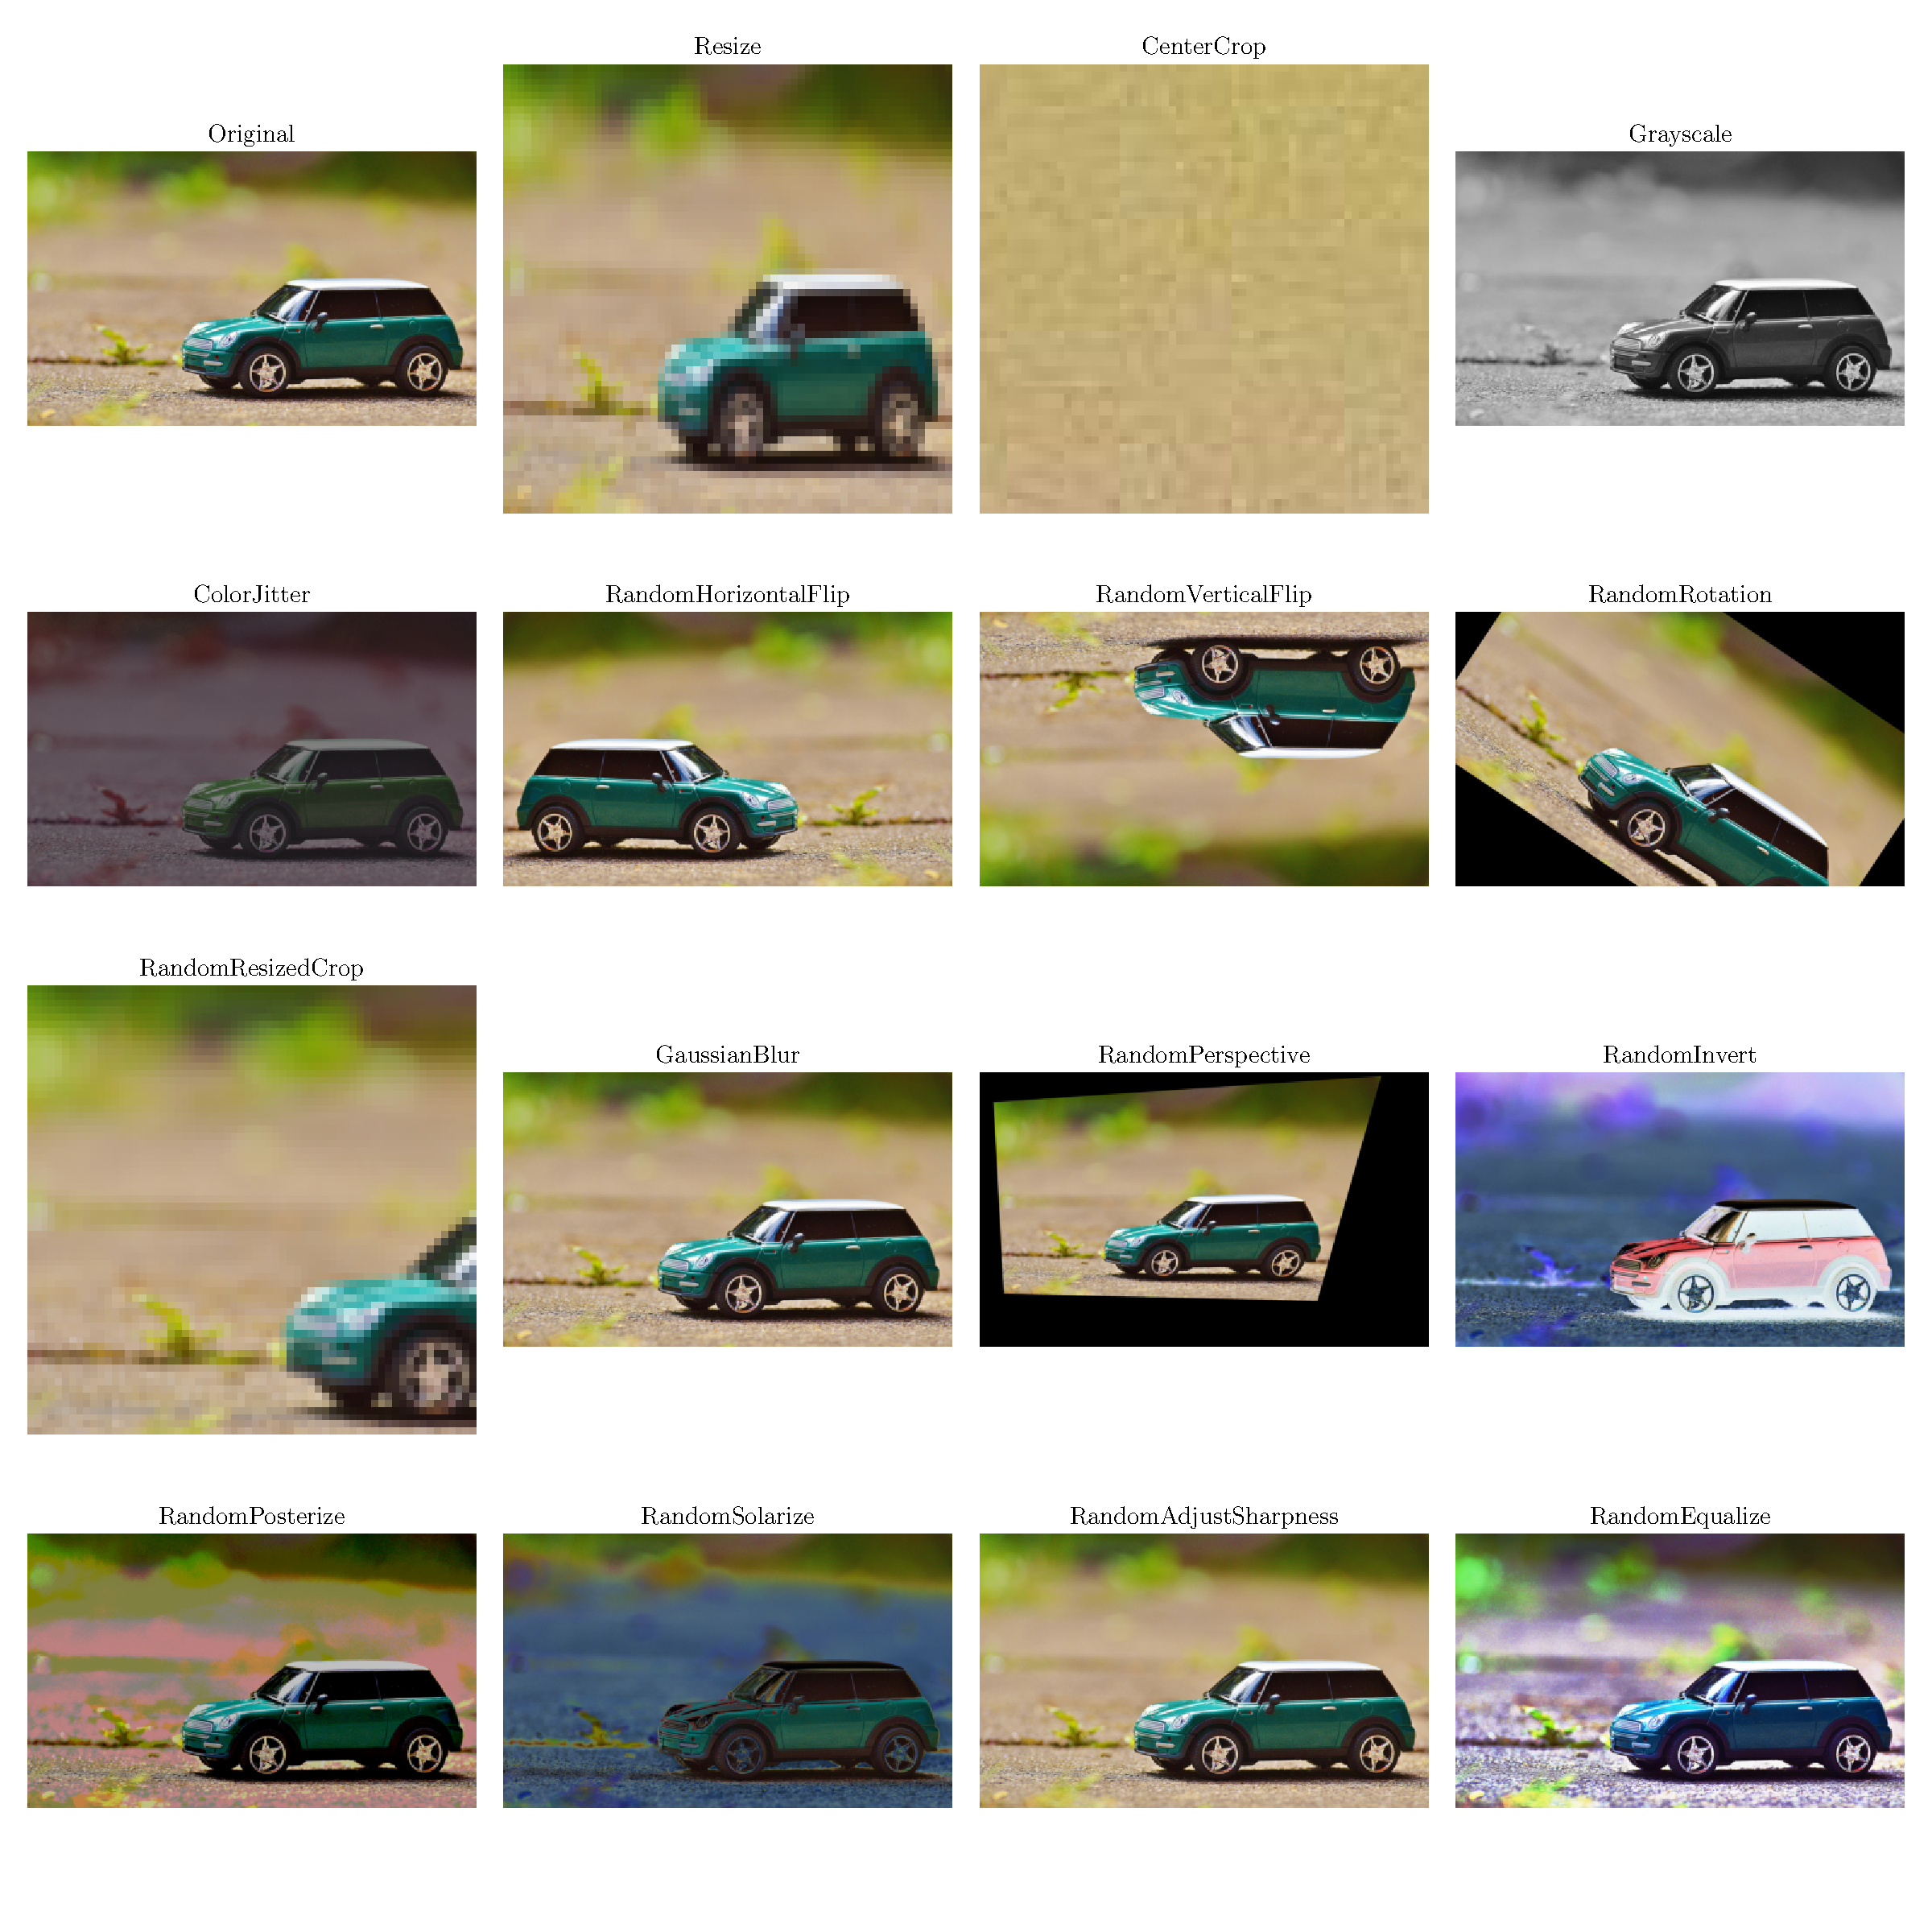
\includegraphics[width=0.8\textwidth]{figures/dataset_augmentation.pdf}
	\caption{Common dataset augmentation transformations.}
	\label{fig:dataset_augmentation}
\end{figure} 
Using dataset augmentation, the model can learn more from the data, because one creates several different augmented versions of each already existing training dataset sample.% Slide 25, Lec 4
}

\Que{How does semi-supervised learning work?}
\Ans{
	Consider the case, where one has labelled samples $\{(x^{(i)},y^{(i)})\}_{i=1,\dots,m}$ and unlabelled samples $\{x^{(j)}\}_{j=m+1,\dots,n}$. This corresponds to the case, where one has labelled some, but not all of the samples in the dataset. This is quite common in application cases, because labelling is very expensive. Semi-supervised learning aims to leverage techniques of unsupervised learning to label the unlabelled data based on the labelled samples. The difference to unsupervised learning is that for a start one knows some samples of the different classes with certainty, because they have been labelled.
	
	The key technique is visualized in \cref{fig:semi_supervised_learning}.
	\begin{figure}[h]
		\centering
		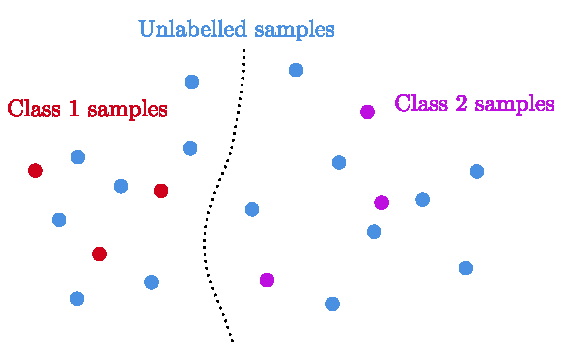
\includegraphics[width=0.4\textwidth]{figures/semi_supervised_learning.pdf}
		\caption{Key idea of semi-supervised learning is to use labelled samples to label unlabelled samples based e.g. on the distance of an unlabelled sample to the nearest labelled sample.}
		\label{fig:semi_supervised_learning}
	\end{figure}
	One common assumption to label the unlabelled samples based on the labelled samples is the so-called cluster assumption, which posits that data points in the same cluster are likely to belong to the same class. For example, one can use a unsupervised clustering technique such as k-means or PCA to cluster the data. One can in a second step assign to each unlabelled sample in the cluster the label the majority of labelled samples in that cluster have. There are a variety of ways on how to label the unlabelled samples based on the labelled samples, but the key idea is always the same.
}

\Que{How does the FixMatch semi-supervised learning technique work?}
\Ans{
The FixMatch semi-supervised learning technique is a special implementation of how to label the unlabelled samples based on the labelled samples in the case, where one has labelled samples $\{(x^{(i)},y^{(i)})\}_{i=1,\dots,m}$ and unlabelled samples $\{x^{(j)}\}_{j=m+1,\dots,n}$.

Consider \cref{fig:fixmatch} to study the working principle of the FixMatch algorithm.
\begin{figure}[h]
	\centering
	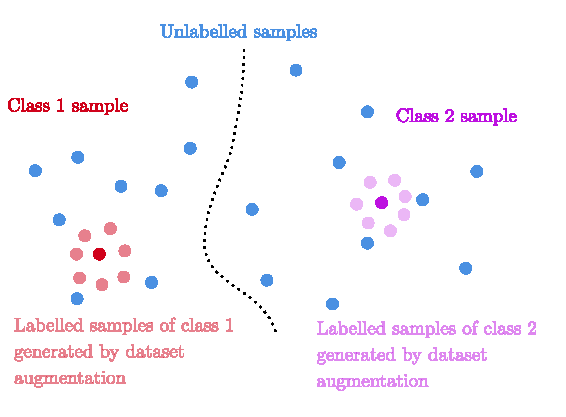
\includegraphics[width=0.4\textwidth]{figures/fixmatch.pdf}
	\caption{FixMatch algorithm working principle.}
	\label{fig:fixmatch}
\end{figure}
First, the model is trained on the labelled samples (strong red and purple points in \cref{fig:fixmatch}). Then, the labelled samples are augmented such that one obtains various new labelled samples. Those obtained new samples by means of dataset augmentation can be labelled because one knows from which labelled sample they were generated. The model is retrained on the orignially labelled samples and on labelled samples by dataset augmentation (weak red and puple points in \cref{fig:fixmatch}). Then, the model is used to make label predictions on the unlabelled samples in the dataset. These predictions are of a probabilistic nature; hence one can set a threshold to classify an unlabelled sample with the most likely class. All the unlabelled samples that exceed that threshold are labelled in this way - they are known then as pseudo-labels. Based on the new labelled dataset, one again augments all labelled samples and retrains the model on it. Then, again predictions on unlabelled samples are made and classified with the most likely label, if the threshold is met. This procedure is repeated until all of the unlabelled samples are labelled. Then, a normal classifying network can be trained on the whole dataset.
}

\Que{What is multi-task learning and what can be the issue with training such algorithms?}
\Ans{
	Multi-task learning (MTL) is a regularization technique in whic a model is trained on multiple related tasks simultaneously, sharing representations among them to improve generalization. Formally, for tasks $ T_1, T_2, \ldots, T_n$ and associated predictive functions $f_k(x;\theta)$ based on the shared parameters $\theta$ and input $x$, MTL aims to minimize the total loss
	\begin{equation}
	\min_\theta \sum_{k=1}^n \lambda_k \mathcal{L}_k(f_k(x; \theta)),
\end{equation}
	where $\mathcal{L}_k$ is the loss for task $T_k$ and $\lambda_k$ are the task-specific weighting coefficients to allow for different importances of tasks. 
	
	A major issue with MTL is so-called negative transfer, where learning one task degrades performance on another due to conflicting gradients or task incompatibility. Proper balancing of task-specific losses (\( \lambda_k \)) and architectural decisions (e.g., what to share) is crucial.
}

\Que{What is deep double descent?}
\Ans{
	Deep double descent describes the non-monotonic behavior of generalization error as a function of model complexity. Traditionally, the bias-variance tradeoff suggests a U-shaped curve. For too little model complexity, the model makes too strong assumptions, e.g. linearity and hence has a high bias and does not generalize well. At a sweet spot, one has an ideal tradeoff between bias and variance in the model. If the model is chosen too complex, one classically expects a rise again in the generalization error, because the model has started to fit the noise in the data and hence the model has too much variance.
	\begin{figure}[h]
		\centering
		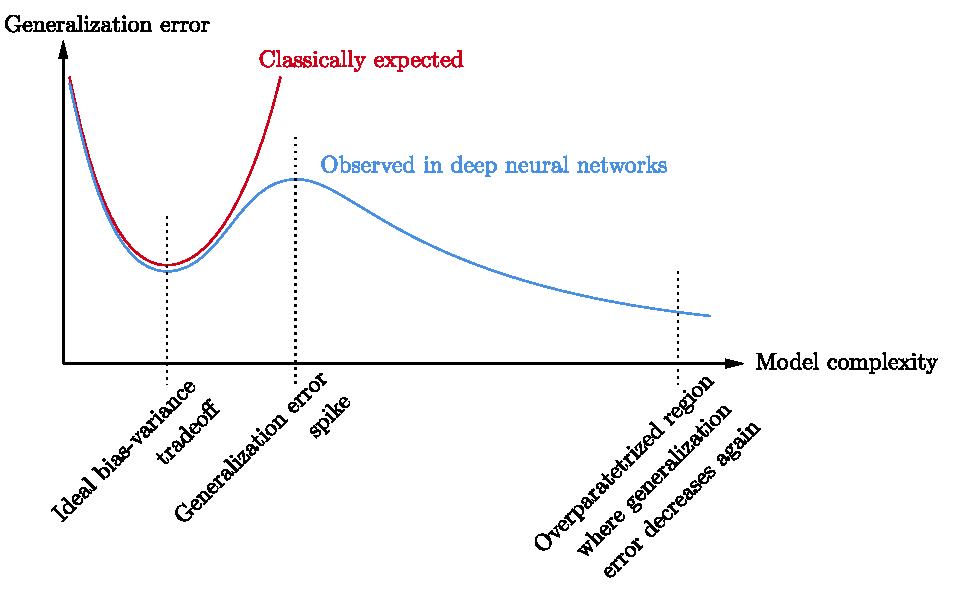
\includegraphics[width=0.5\textwidth]{figures/ddd.pdf}
		\caption{Deep double descent visualization.}
		\label{fig:ddd}
	\end{figure}
	
	Neural networks however show a surprising behaviour sometimes: The generalization error decreases again, if the model is chosen sufficiently complex; see \cref{fig:ddd} for a visualization of this. This is known as deep double descent. In deep learning therefore, it is sometimes better to have a very large model, because with respect to the classically best tradeoff between variance and bias, it can achieve an even better generalization error. This is counterintuitive but explains why very large models can still generalize well despite having capacity to overfit. The deep double descent (when the generalization decreases the second time after a local maximum) typically occurs at larger model complexities than where the training error would be nearly zero.
}

\Que{How can early stopping of training be viewed as another kind of regularization technique?}
\Ans{
	Early stopping is a regularization technique that stops training a model when its performance on a separate validation set stops getting better. This helps prevent overfitting, which happens when the model learns the training data too well - including its noise and random errors—and performs poorly on new, unseen data.
	
	Even though early stopping does not directly change the loss function like other regularization methods, it has a similar effect. When training a model using gradient descent
	
	\begin{equation}
	\theta_{t+1} = \theta_t - \eta \nabla \mathcal{L}(\theta_t),
	\end{equation}
	the parameters \( \theta \) are updated in steps. If we stop early, we prevent \( \theta \) from growing too large or fitting the training data too perfectly. This is similar to what L2-regularization (like ridge regression) does: It keeps the parameter values small to avoid overfitting.
	
	So, early stopping acts like an indirect form of regularization by limiting how much the model can adapt to the training data.
}

\Que{How does the parameter sharing regularization technique work?}
\Ans{
	Parameter sharing enforces that multiple parts of the model use the same parameters. A classic example is convolutional neural networks (CNNs), where filters (kernels) are shared across spatial locations. This reduces the number of parameters and improves generalization.
}

\Que{How does imposing sparsity for neural network representation help as regularization?}
\Ans{
	Sparsity regularization encourages the network to use fewer neurons or connections, reducing overfitting and enhancing interpretability. This is commonly achieved using \( L_1 \) regularization on weights or activations:
	
	\[
	\mathcal{L}_{\text{total}} = \mathcal{L}_{\text{data}} + \lambda \|\theta\|_1
	\]
	
	Alternatively, a sparsity penalty can be added to the hidden activations, e.g., KL-divergence between average activation and a small target \( \rho \):
	
	\[
	\sum_j \text{KL}(\rho \| \hat{\rho}_j) = \sum_j \rho \log \frac{\rho}{\hat{\rho}_j} + (1-\rho) \log \frac{1-\rho}{1-\hat{\rho}_j}
	\]
	
	This encourages the model to activate only a small subset of neurons, limiting capacity and promoting generalization.
}

\Que{What are L1- and L2-regularization and what is the key difference?}
\Ans{
	L1- and L2-regularization are techniques used in machine learning to reduce overfitting by penalizing large model weights, which encourages simpler and more generalizable models.
	
	Let $\mathcal{L}_{base}$ be a base loss function such as cross-entropy loss, the mean squared loss (MSE) or just the negative log-likelihood of the data given the model parameters $\theta$. L1- and L2-regularization add an additional term to the base loss function in order to penalize large model weights, which has the result that simpler models are encouraged and thus allow the model to generalize better.
	
	In L1-regularization (lasso regression), the added regularization term is the norm of the model weights $\theta$ scaled by a weighting factor $\lambda$, namely \begin{equation}
		\mathcal{L}_{tot} = \mathcal{L}_{base} + \lambda \|\theta\|_1
	\end{equation} where $\|\theta\|_1 = \sum_{j}|\theta_j|$. L1-regularization tends to drive some weights exactly to zero, resulting in sparse models that can perform feature selection.
	
	In L2-regularization (ridge regression), the added regularization is the norm squared of the
	the model weights $\theta$ scaled by a weighting factor $\lambda$, namely \begin{equation}
		\mathcal{L}_{tot} = \mathcal{L}_{base} + \lambda \|\theta\|^2,
	\end{equation} where $\|\theta\|_2 = \sqrt{\sum_{j}\theta_j^2}$. L2-regularization discourages large weights by adding a quadratic penalty. This leads to smaller, but typically nonzero weights and hence non-sparse models.

The key differences between L1- and L2-regularization are the following:
	\begin{itemize}
		\item L2-regularization spreads the penalty across all weights, leading to smaller but nonzero values.
		\item L1-regularization focuses the penalty in a way that some weights are shrunk entirely to zero, promoting sparsity.
	\end{itemize}
}

\Que{What does sparsity mean with respect to deep learning or with matrices in general?}
\Ans{
Sparsity means that most elements of the mathematical object under consideration are zero. With respect to the parameters of a neural network, sparsity means that many of the weights parametrizing the network are exactly zero. Encouraging sparsity can lead to better generalization properties. With respect to matrices, a matrix is called sparse if many or most of the matrix elements are zero.
}

\Que{How does ensembling of methods/datasets improve the generalization properties of a neural network?}
\Ans{
		Consider a number of random variables $x_1,\dots,x_n$ with associated variances $\sigma_{x_i}^2\doteq \mathbb{V}(x_i)$ for $i=1,\dots,n$. Now, if each random variable $x_i$ is understood a the prediction of the $i$'th model, it is reasonable to compute an average prediction $\bar{x}$ as \begin{equation}
			\bar{x} = \frac{1}{n}\sum_{i=1}^{n}x_i.
		\end{equation} It is now interesting to calculate the variance $\mathbb{V}(\bar{x})$ on the average prediction $\bar{x}$. Doing this, we obtain
		\begin{align}
			\begin{aligned}
				\sigma_{\bar{x}}^2 &\doteq \mathbb{V}(\bar{x}) = \mathbb{V}\left(\frac{1}{n}\sum_{i=1}^n x_i\right) = \mathbb{E}\left[\left(\frac{1}{n}\sum_{i=1}^{n}x_i - \mathbb{E}\left[\frac{1}{n}\sum_{i=1}^n x_i\right]\right)^2\right] \\
				&=\mathbb{E}\left[\left(\frac{1}{n}\sum_{i=1}^{n}x_i - \frac{1}{n}\sum_{i=1}^n \mathbb{E} [x_i]\right)^2\right] = \mathbb{E}\left[\frac{1}{n^2}\left(\sum_{i=1}^{n}\left(x_i-\mathbb{E}[x_i]\right)\right)^2\right] \\
				&= \frac{1}{n^2}\mathbb{E}\left[\sum_{i=1}^{n}(x_i-\mathbb{E}[x_i])\sum_{j=1}^n(x_j-\mathbb{E})[x_j])\right] = \frac{1}{n^2}\mathbb{E}\left[\sum_{i,j=1}^n(x_i-\mathbb{E}[x_i])(x_j-\mathbb{E}[x_j])\right] \\
				&= \frac{1}{n^2}\mathbb{E}\left[\sum_{i=1}^{n}(x_i-\mathbb{E}[x_i])^2 + 2\sum_{1\leq i < j \leq n}(x_i-\mathbb{E}[x_i])(x_j-\mathbb{E}[x_j])\right] \\
				&= \frac{1}{n^2}\left(\sum_{i=1}^{n}\mathbb{E}\left[(x_i-\mathbb{E}[x_i])^2\right] + 2\sum_{1\leq i < j \leq n}\mathbb{E}\left[(x_i-\mathbb{E}[x_i])(x_j-\mathbb{E}[x_j])\right]\right) \\
				&= \frac{1}{n^2}\left(\sum_{i=1}^{n}\mathbb{V}(x_i)+ 2\sum_{1\leq i < j \leq n}\mathbb{K}(x_i,x_j)\right) = \frac{1}{n^2}\sum_{i=1}^{n}\sigma_{x_i}^2 + \frac{2}{n^2}\sum_{1\leq i < j \leq n} \rho(x_i,x_j)\sigma_{x_i}\sigma_{x_j},
			\end{aligned} 
		\end{align} where $\rho(x_i,x_j)$ is the correlation coefficient defined by \begin{equation}
			\rho(x_i,x_j) = \frac{\mathbb{K}(x_i,x_j)}{\sqrt{\mathbb{V}(x_i)\mathbb{V}(x_j)}},
		\end{equation} which is evidently zero, if the covariance is zero. For perfect correlation or anticorrelation, the correlation coefficient is either $+1$ or $-1$, so $\rho(x_i,x_j) \in [-1,1]$.
		
		Consider the case, where the random variables are identically distributed with correlation coefficient $\rho$, i.e. $\sigma_{x_i} = \sigma$ for all $i=1,\dots,n$. Then, the variance $\sigma_{\bar{x}}$ on the mean $\bar{x}$ is given by \begin{align}\begin{aligned}
				\sigma_{\bar{x}}^2 &=\frac{1}{n^2}\sum_{i,j=1}^{n}\mathbb{E}\left[(x_i-\mathbb{E}[x_i])(x_j-\mathbb{E}[x_j])\right] = \frac{1}{n^2}\sum_{i,j=1}^{n}\mathbb{K}(x_i,x_j) \\ &= \frac{1}{n^2}\left(\sum_{i=1}^{n}\mathbb{V}(x_i)+\sum_{\substack{i,j=1 \\ i\neq j}}^{n}\mathbb{K}(x_i,x_j)\right) = \frac{n\sigma^2}{n^2}+ \frac{1}{n^2}\sum_{\substack{i,j=1 \\ i\neq j}}^{n}\rho \sqrt{\mathbb{V}(x_i)\mathbb{V}(x_j)} \\ &= \frac{n\sigma^2}{n^2} + \frac{n(n-1)}{n^2}\rho\sigma^2 = \rho\sigma^2 + \frac{\sigma^2(1-\rho)}{n}.
		\end{aligned}\end{align} And if it is the case that the random variables are furthermore identically and independently distributed, we have $\rho=0$ because of the correlations being zero, meaning that \begin{equation}
			\sigma_{\bar{x}}^2 = \frac{\sigma^2}{n}.
		\end{equation}
		
		The general idea behind ensembling methods is therefore to find several models to make a prediction on the same sample; these predictions can be denoted by the random variables $x_1,\dots,x_n$. Depending on the correlation $\rho(x_i,x_j)=\frac{\mathbb{K}(x_i,x_j)}{\sqrt{\mathbb{V}(x_i)\mathbb{V}(x_j)}}$ between the models and the variances $\mathbb{V}(x_i)$, the resulting average prediction given by $\bar{x} = \frac{1}{n}\sum_{i=1}^nx_i$ will have a lower variance than the lowest of all predictions; it can however also be larger, this entirely depends on the incoming variances and correlations. In general therefore, in order to achieve a better performance of the ensembled method in comparison to individual methods, one needs to decrease correlation (decrease $\rho$) between models aswell as provide as many models as possible (increase $n$).
}

\Que{How does dropout help to improve generalization properties of a neural network?}
\Ans{
	Dropout is a regularization technique that improves generalization by randomly deactivating a subset of neurons during training. This prevents the network from becoming too reliant on any particular subset of features or neurons, encouraging redundancy and robustness.
}

\Que{How do adversarial samples help for generalization of a model?}
\Ans{
	Adversarial training improves generalization by exposing the model to intentionally perturbed inputs designed to challenge its robustness. These adversarial examples are generated by adding a small but worst-case perturbation 
	\begin{equation}
		x_{adv} = x + \epsilon  \text{sign}(\nabla_x \mathcal{L}),
	\end{equation}
	to the input \( x \), often in the direction of the gradient of the loss as in this formula. Here, \( \epsilon \) controls the size of the perturbation, and \( \mathcal{L} \) is the loss function. The function \( \text{sign}(\cdot) \) returns the sign of each component of the gradient, i.e.,
	\begin{equation}
	\text{sign}(z_i) =
	\begin{cases}
		-1 & \text{if } z_i < 0 \\
		0 & \text{if } z_i = 0 \\
		1 & \text{if } z_i > 0
	\end{cases}
\end{equation}
	applied element-wise. This ensures that the perturbation has a fixed magnitude in each dimension, corresponding to the direction that most increases the loss.
	
	Training on such hard examples forces the model to learn decision boundaries that are not only accurate but also more robust to small input variations. As a result, the model becomes less sensitive to noise and spurious patterns, leading to better generalization.
}

\subsection{Optimization}

\Que{Why are mini-batches or batches of data used for training a neural network?}
\Ans{
	It is computationally expensive, to compute and backpropagate the loss on the whole training set at each iteration. This is known as just gradient descent - it works by calculating the gradient of the loss function with respect to the model weights, given as input all the samples from the training dataset. In order to make the training process more efficient, one can use just a small subset of samples from the training dataset, for which the gradients are calculated - this is known as mini-batch gradient descent and is referred also to stochastic gradient descent. % Slides 7ff, lec 5
}

\Que{How are saddle points of loss functions an issue in optimization of neural networks and what are the strategies to overcome them?}
\Ans{
	Saddle points occur in non-convex loss spaces and are very common in the field of neural networks. At saddle points, the gradient is zero, but those points are neither local minima nor local maxima. In high-dimensional spaces, saddle points are much more common than local minima. At a saddle point, the Hessian matrix of second derivatives has both positive and negative eigenvalues, meaning there are directions of both increasing and decreasing curvature. The problem with saddle points is that they can cause optimization algorithms to stagnate or slow down.
	
	To overcome this issue, the following strategies are commonly employed:
	\begin{itemize}
		\item Stochastic gradient descent: The inherent noise in SGD helps escape saddle points by perturbing the updates and allowing the optimizer to move away from flat regions.
		\item Adaptive learning rate: Optimizers like RMSProp, Adam, or Adagrad adjust the learning rate per parameter based on recent gradient information, helping to avoid slow convergence near saddle points.
		\item Add momentum: Momentum-based methods help carry the parameters through flat regions of the loss surface, thus escaping saddle points faster.
	\end{itemize}
}

\Que{What are the basic optimization algorithms and how do they work?}
\Ans{
	The basic optimization algorithms used in training neural networks aim to minimize a loss function \( J(\theta) \) with respect to the model parameters \( \theta \), given some training data samples. The most common algorithms include:
	
	\begin{itemize}
		\item \textbf{Gradient descent:}
		\begin{equation}
		\theta_{t+1} = \theta_t - \alpha \nabla_\theta J(\theta_t),
		\end{equation}
		where \( \alpha \) is the learning rate. The update is based on the full dataset and is computationally expensive.
		
		\item \textbf{Stochastic gradient descent (SGD):} Instead of computing the gradient over the full dataset, SGD approximates it using a single or mini-batch of examples:
		\begin{equation}
		\theta_{t+1} = \theta_t - \alpha \nabla_\theta J_{\mathcal{B}}(\theta_t),
		\end{equation}
		where \( \mathcal{B} \) is a mini-batch. It introduces noise but speeds up computation and can escape local minima.
		
		\item \textbf{Momentum:}
		\begin{equation}
		v_{t+1} = \beta v_t + \nabla_\theta J(\theta_t), \quad \theta_{t+1} = \theta_t - \alpha v_{t+1},
		\end{equation}
		where \( \beta \in [0,1) \) is a momentum coefficient. Momentum helps accelerate updates in the correct direction.
		
		\item \textbf{RMSProp:}
		\begin{equation}
		s_t = \rho s_{t-1} + (1 - \rho)(\nabla_\theta J(\theta_t))^2, \quad \theta_{t+1} = \theta_t - \frac{\alpha}{\sqrt{s_t + \varepsilon}} \nabla_\theta J(\theta_t),
		\end{equation}
		which adapts the learning rate to each parameter.
		
		\item \textbf{Adam:} Combines momentum and RMSProp:
		\begin{equation}
		m_t = \beta_1 m_{t-1} + (1 - \beta_1)\nabla_\theta J(\theta_t), \quad
		v_t = \beta_2 v_{t-1} + (1 - \beta_2)(\nabla_\theta J(\theta_t))^2,
		\end{equation}
		\begin{equation}
		\hat{m}_t = \frac{m_t}{1 - \beta_1^t}, \quad \hat{v}_t = \frac{v_t}{1 - \beta_2^t}, \quad
		\theta_{t+1} = \theta_t - \alpha \frac{\hat{m}_t}{\sqrt{\hat{v}_t} + \varepsilon}.
		\end{equation}
	\end{itemize}
	Each method attempts to balance speed, stability, and adaptability during the optimization process.
}

\Que{What is batch normalization and how does it work? What are the cases where batch normalization does not work well and why?}
\Ans{
	Batch normalization aims to improve the stability and speed of neural network training by normalizing layer inputs across a mini-batch. Given a mini-batch \( \mathcal{B} = \{x^{(1)}, \ldots, x^{(m)}\} \), the mean and variance are computed as
	
	\begin{equation}
		\mu_\mathcal{B} = \frac{1}{m} \sum_{i=1}^m x^{(i)}, \quad \sigma^2_\mathcal{B} = \frac{1}{m} \sum_{i=1}^m (x^{(i)} - \mu_\mathcal{B})^2.
	\end{equation}
	
	Then, each input is normalized and scaled:
	
	\begin{equation}
		\hat{x}^{(i)} = \frac{x^{(i)} - \mu_\mathcal{B}}{\sqrt{\sigma^2_\mathcal{B} + \varepsilon}}, \quad y^{(i)} = \gamma \hat{x}^{(i)} + \beta,
	\end{equation}
	where \( \gamma \) and \( \beta \) are learnable parameters. This transformation ensures consistent distributions across training and helps reduce internal covariate shift.
	
	However, batch normalization has some limitations:
	
	\begin{itemize}
		\item It is less effective when batch sizes are very small, as the statistics become noisy.
		\item It is difficult to apply in online learning or reinforcement learning where mini-batches are not available.
		\item In recurrent neural networks, temporal dependencies make batch normalization harder to integrate without disrupting sequence modeling.
	\end{itemize}
}

\Que{What is coordinate descent and how does it work?}
\Ans{
	Coordinate descent is an optimization technique that updates one parameter at a time, while holding all others fixed. Suppose the parameter vector is \( \theta = (\theta_1, \ldots, \theta_n)^\top \). At each iteration, one selects a coordinate \( j \) and solves
	
	\begin{equation}
		\theta_j \leftarrow \arg\min_{\theta_j} \left[J(\theta_1, \ldots, \theta_{j-1}, \theta_j, \theta_{j+1}, \ldots, \theta_n)\right].
	\end{equation}
	
	This method is especially efficient when each coordinate-wise minimization can be computed quickly or in closed form. Coordinate descent is particularly useful in problems with sparsity-inducing regularizers, such as lasso regression. That is because of there are many weights exactly equal to zero (sparsity), then only a few non-zero parameters survive and hence only for these, a gradient must be calculated. This is then efficiently done by coordinate descent.
}

\Que{What is weight averaging and how does it work?}
\Ans{
	Weight averaging is a regularization technique where the final model parameters are taken as the average over multiple checkpoints during training. This technique is known to improve generalization and flatten the effective loss landscape.
	
	Suppose the parameters \( \theta^{(t)} \) are obtained at iteration \( t \), the averaged weights over \( T \) iterations are given by
	
	\begin{equation}
		\bar{\theta} = \frac{1}{T} \sum_{t=1}^T \theta^{(t)}.
	\end{equation}
	
	This approach, often called stochastic weight averaging, leads to solutions that lie in wider optima of the loss function, which have been empirically linked to better generalization performance. Weight averaging can be implemented efficiently and requires no change to the training loop apart from storing and averaging parameters during later training epochs.
}

\section{Convolutional neural networks}
\Que{What is a feature of some object?}
\Ans{
	A feature is an independent, explanatory factor that captures a specific property or characteristic of an object. In the context of deep learning, features are typically derived from raw data \( x \) by applying transformation functions \( \phi_j(x) \). Each feature \( \phi_j(x) \) represents a learned aspect of the input, such as edges, textures, or shapes in image data. The deep network then builds hierarchical representations by learning increasingly abstract features in successive layers.
}

\Que{What is the general architecture of a deep learning network and are the purposes of the different parts?}
\Ans{
	A typical deep learning network consists of an input layer, multiple hidden layers, and an output layer. Each layer applies a function \( f(x^{(i)}; \theta) \), parameterized by weights \( \theta \), to the outputs of the previous layer. The overall structure is:
	
	\begin{equation}
		f(x) = f^{(L)} \circ \cdots \circ f^{(2)} \circ f^{(1)}(x),
	\end{equation}
	where \( f^{(l)} \) denotes the function applied at layer \( l \), and \( L \) is the total number of layers. The input layer receives raw data \( x \), hidden layers learn intermediate features, and the output layer produces the final prediction (e.g., class probabilities). Each layer often includes a linear transformation followed by a nonlinear activation function.
}

\Que{How does a typical convolutional neural network look like and what are the purposes of the different parts?}
\Ans{
	A typical convolutional neural network (CNN) is composed of several key components (see \cref{fig:cnn}):
	
	\begin{itemize}
		\item \textbf{Convolutional layers:} Apply learnable filters to local regions of the input, extracting spatially localized features such as edges or textures.
		\item \textbf{Activation functions:} Introduce nonlinearity into the network (commonly ReLU), enabling the model to learn complex patterns.
		\item \textbf{Pooling layers:} Reduce spatial dimensions while preserving the most important information, providing translation invariance and reducing computational cost.
		\item \textbf{Fully connected layers:} Often appear at the end of the network and aggregate the learned features to produce final predictions.
	\end{itemize}
	
	Each layer in a CNN contributes to building a hierarchical representation of the input, from low-level features to high-level semantic concepts.\begin{figure}[h]
		\centering
		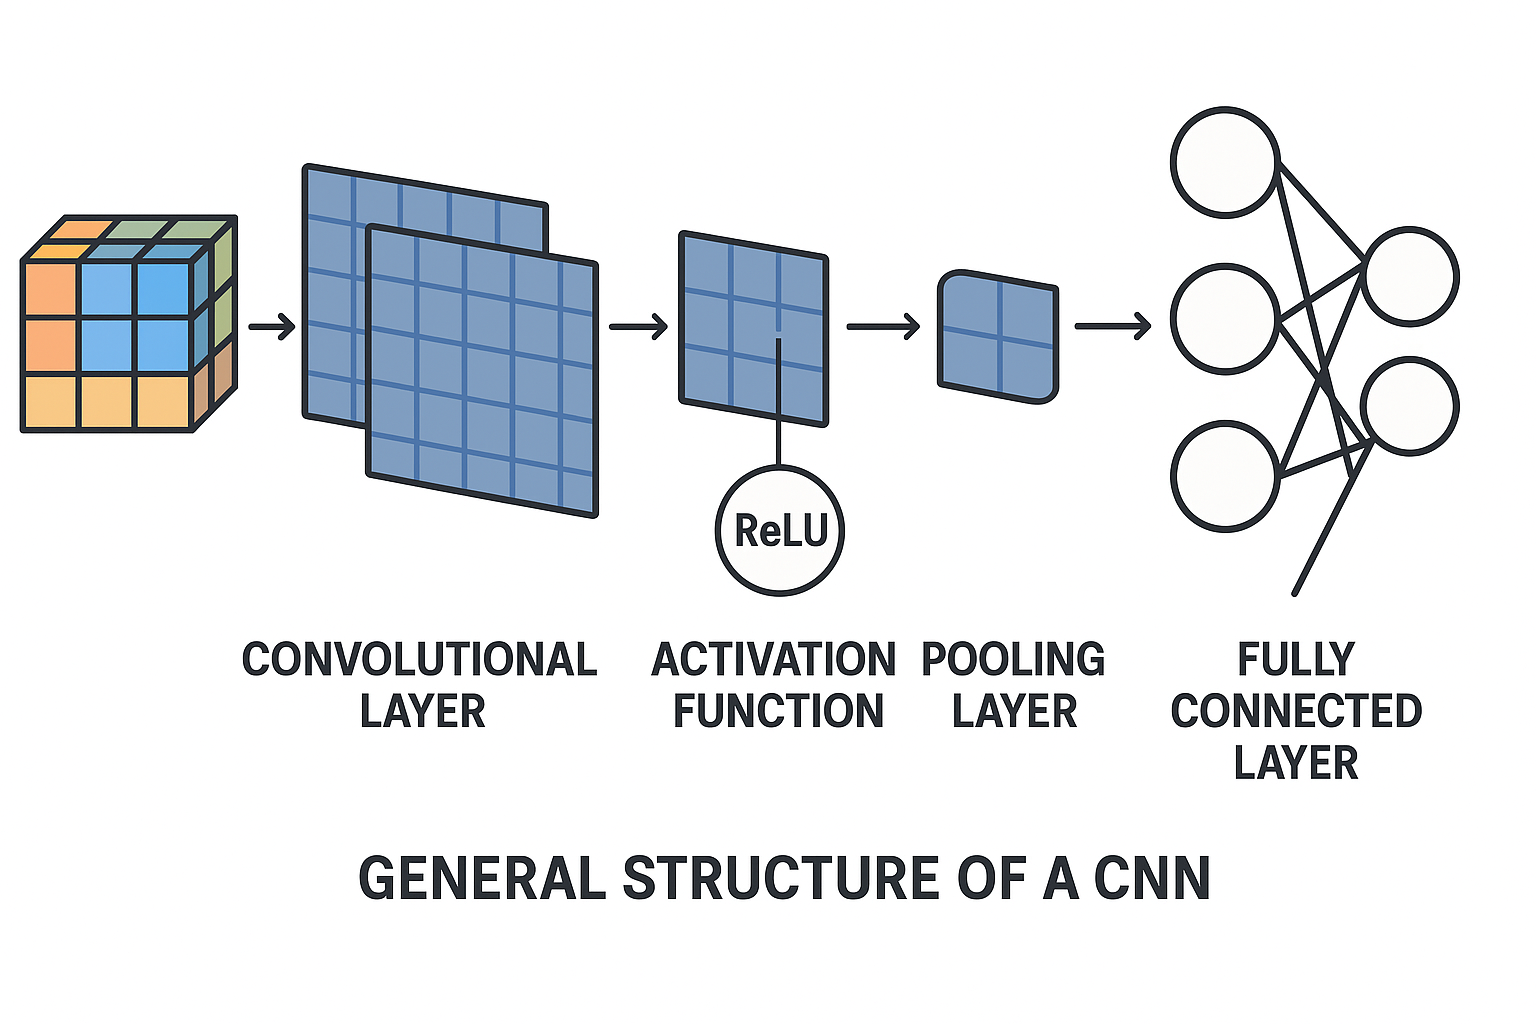
\includegraphics[width=0.5\textwidth]{figures/cnn.png}
		\caption{Visualization of the general architecture of a convolutional neural network (CNN).}
		\label{fig:cnn}
	\end{figure}
}

\Que{How is the convolution operation on a continuous domain defined mathematically and what does it mean?}
\Ans{
	The convolution of two continuous functions \( f(t) \) and \( g(t) \) is defined as:
	
	\begin{equation}
		(f * g)(t) = \int_{-\infty}^{\infty} f(\tau)g(t - \tau) \, \mathrm{d}\tau.
	\end{equation}
	
	This operation represents a weighted integration of the function \( f \) over a shifted and flipped version of the function \( g \). It is used to analyze how one function modifies or filters another and is central to signal processing and systems analysis.
}

\Que{How is the convolution operation on a discrete domain defined mathematically and what does it mean?}
\Ans{
	For discrete signals \( f[n] \) and \( g[n] \), the convolution is defined as:
	
	\begin{equation}
		(f * g)[n] = \sum_{k = -\infty}^{\infty} f[k] \cdot g[n - k].
	\end{equation}
	
	In the context of neural networks, the discrete convolution represents the summation of element-wise products between a kernel (filter) and a patch of the input signal. It is used to detect patterns such as edges or textures in data like images.
}

\Que{How is the correlation operation on a continuous domain defined mathematically and what does it mean?}
\Ans{
	The correlation of two continuous functions \( f(t) \) and \( g(t) \) is defined as:
	
	\begin{equation}
		(f \star g)(t) = \int_{-\infty}^{\infty} f(\tau)g(t + \tau) \, \mathrm{d}\tau.
	\end{equation}
	
	In contrast to convolution, the filter \( g \) is not flipped in correlation. Correlation measures the similarity between the input and a filter across different positions and is commonly used in template matching.
}

\Que{How is the correlation operation on a discrete domain defined mathematically and what does it mean?}
\Ans{
	For discrete signals \( f[n] \) and \( g[n] \), the correlation is defined as:
	
	\begin{equation}
		(f \star g)[n] = \sum_{k = -\infty}^{\infty} f[k] \cdot g[n + k].
	\end{equation}
	
	Correlation slides the kernel over the input without flipping it. In neural networks, although the term convolution is used, what is often implemented is actually correlation.
}

\Que{How do the convolution and correlation operations for images used with convolutional neural networks look like? What is the meaning of the different terms?}
\Ans{
	In the context of convolutional neural networks (CNNs), convolution and correlation are operations that apply a small filter (kernel) to an input image or feature map to extract local patterns.

For a discrete 2D input image \( I \in \mathbb{R}^{H \times W} \) and a kernel \( K \in \mathbb{R}^{k_H \times k_W} \), the discrete 2D convolution is defined as:

	\begin{equation}
		(S * K)(i, j) = \sum_{m=0}^{k_H - 1} \sum_{n=0}^{k_W - 1} K(m, n) \cdot S(i - m, j - n),
	\end{equation}
	where \( S(i, j) \) is the input signal (e.g., an image), \( K \) is the kernel, and the operation slides the flipped kernel across the input. The result is a feature map that reflects how well the kernel pattern matches the input locally.
	
	In practice, deep learning libraries often implement the cross-correlation operation instead of convolution, which is defined as:
	
	\begin{equation}
		(S \star K)(i, j) = \sum_{m=0}^{k_H - 1} \sum_{n=0}^{k_W - 1} K(m, n) \cdot S(i + m, j + n).
	\end{equation}
	This operation does not flip the kernel and is computationally simpler. Despite this, it is still referred to as ``convolution'' in most CNN implementations. The individual terms in the cross-correlation and convolution operations mean the following:
	\begin{itemize}
		\item \( S(i,j) \): The pixel value at position \( (i,j) \) of the input image or feature map.
		\item \( K(m,n) \): The filter coefficient at position \( (m,n) \) of the kernel.
		\item \( (i,j) \): The current location of the kernel center over the input.
		\item The sums: Perform element-wise multiplications between the kernel and the overlapping input patch, then add the results to produce one pixel of the output.
	\end{itemize}
	
	Both convolution and correlation are used to compute feature maps that represent the activation of specific patterns (e.g., edges, textures) across the input. These maps are then passed through activation functions and pooled, contributing to the hierarchical feature representation in CNNs.
}


\Que{How can a fully connected layer be understood as a special case of a convolutional layer? What is the Toeplitz matrix in this regard?}
\Ans{
	A fully connected (dense) layer can be viewed as a special case of a convolutional layer where the following hold:
	\begin{itemize}
		\item The input is a one-dimensional signal (or flattened).
		\item The convolutional filter spans the entire input (i.e., the kernel size equals the input size).
		\item The stride is 1 and no padding is used.
		\item There is only one receptive field, meaning the output is a single neuron.
	\end{itemize}
	In this case, the convolution effectively becomes a dot product between the input and the filter, which is exactly what a fully connected layer performs (plus a bias term in the case of a fully connected layer).
	
	To see this more generally, we can represent a 1D convolution as a matrix-vector multiplication. Suppose the input \( x \in \mathbb{R}^n \) and the kernel \( k \in \mathbb{R}^m \), the convolution operation can be written as
	\begin{equation}
		y = T x,
	\end{equation}
	where \( y \in \mathbb{R}^{n - m + 1} \) and \( T \in \mathbb{R}^{(n - m + 1) \times n} \) is a Toeplitz matrix. The Toeplitz matrix has a special structure: each descending diagonal from left to right is constant. For example, for \( n = 5 \) and \( m = 3 \), the convolution kernel \( k = [k_1, k_2, k_3] \) gives rise to the matrix
	\begin{equation}
		T = 
		\begin{bmatrix}
			k_1 & k_2 & k_3 & 0   & 0 \\
			0   & k_1 & k_2 & k_3 & 0 \\
			0   & 0   & k_1 & k_2 & k_3
		\end{bmatrix}.
	\end{equation}
	The convolution output is then:
	\begin{equation}
		y = T x = 
		\begin{bmatrix}
			k_1 x_1 + k_2 x_2 + k_3 x_3 \\
			k_1 x_2 + k_2 x_3 + k_3 x_4 \\
			k_1 x_3 + k_2 x_4 + k_3 x_5
		\end{bmatrix}.
	\end{equation}
	In contrast, a fully connected layer computes
	\begin{equation}
		y = W x + b,
	\end{equation}
	where \( W \in \mathbb{R}^{d \times n} \) is an arbitrary weight matrix with no structural constraints, and \( b \) is a bias vector. The key difference is that convolution enforces weight sharing and locality (i.e., the kernel slides across the input), which is reflected in the structured Toeplitz form of \( T \), whereas a fully connected layer learns independent weights for every input-output pair.
}


\Que{What are the key ideas of convolutional layers?}
\Ans{
	The key ideas of convolutional layers are:
	\begin{itemize}
		\item \textbf{Local connectivity:} Each neuron is connected only to a small, localized region of the input. This means that a convolutional neuron located at position $(i,j)$ in the output feature map only processes a small receptive field from the input given by the kernel size.
		\item \textbf{Parameter sharing:} The same set of weights (filter) is applied across all spatial locations, drastically reducing the number of parameters.
		\item \textbf{Translation equivariance:} A shift in the input leads to a corresponding shift in the output feature map, preserving spatial structure.
	\end{itemize}
	These principles enable convolutional layers to efficiently extract meaningful features from high-dimensional data such as images.
}

\Que{What is pooling in the context of convolutional layers and how does it work?}
\Ans{
	Pooling is a downsampling operation that reduces the spatial dimensions of feature maps while preserving the most salient information. Common pooling types include:
	
	\begin{itemize}
		\item \textbf{Max pooling:} Takes the maximum value in each local region.
		\item \textbf{Average pooling:} Computes the average value in each region.
	\end{itemize}
	Mathematically, for a region \( R \subset \mathbb{R}^n \), max pooling outputs:
	\begin{equation}
		y = \max_{x \in R} x.
	\end{equation}
	Pooling provides translation invariance and reduces computational cost by shrinking the size of intermediate representations.
}

\Que{What do the stride and padding parameters of a convolutional layer mean?}
\Ans{
	In convolutional layers, the stride determines how far the filter moves across the input. A stride of 1 means the filter shifts one unit at a time, while a stride of 2 skips every other unit, leading to reduced output resolution.
	
	Padding refers to the addition of extra values (often zeros) around the border of the input. This controls the spatial size of the output and helps preserve the input dimensions. Without padding, the output becomes smaller after each convolution.
}

\Que{What is the general formula relating the different parameters of the convolution operation such as padding and stride with the output size?}
\Ans{
	The output size of a convolution operation is determined by several parameters: Input size $n$ (height or width), kernel size $k$ (height or width), adding $p$ (number of pixels added to each side) and stride $s$ (step size of the kernel). Assuming 1D for simplicity (the 2D case applies this formula along both dimensions), the general formula for the output size \( o \) is
	\begin{equation}
		o = \left[ \frac{n + 2p - k}{s} \right] + 1.
	\end{equation}
}


\section{Deep recurrent neural networks}
\Que{What is the basic difference between convolutional neural networks and recurrent neural networks?}
\Ans{
	While convolutional neural networks (CNNs) are used for processing data with a grid-like topology (e.g., images, which are 2D grids of pixels), recurrent neural networks (RNNs) are designed for handling sequential data, such as time series, text, or speech.
	
	In CNNs, the output at a given location depends only on a local region of the input (local connectivity), and the weights are shared across different spatial locations. In contrast, RNNs incorporate a temporal dimension: The output at time step \( t \) depends on both the input at that time \( x_t \) and the hidden state from the previous time step \( h_{t-1} \). This recursive formulation allows RNNs to model temporal dependencies and internal memory as
	\begin{equation}
		h_t = f(h_{t-1}, x_t).
	\end{equation}
}

\Que{How can a recurrent neural network be defined mathematically?}
\Ans{
	A recurrent neural network (RNN) maintains a hidden state vector \( h_t \in \mathbb{R}^n \) that summarizes the sequence information up to time step \( t \). Given an input sequence \( (x_1, x_2, \dots, x_T) \), the RNN computes
	\begin{equation}
		h_t = \phi(W_{hh} h_{t-1} + W_{xh} x_t + b_h), \qquad y_t = W_{hy} h_t + b_y,
	\end{equation}
	where \( \phi \) is a nonlinear activation function, typically \( \tanh \) or \( \text{ReLU} \), \( W_{xh}, W_{hh}, W_{hy} \) are weight matrices and \( b_h, b_y \) are bias terms. This recurrence allows the model to retain memory of previous inputs via the hidden state.
}

\Que{What are recurrent neural networks (RNN) and what are they used for?}
\Ans{
	Recurrent neural networks are a class of neural networks specifically designed for modeling sequences. Unlike feedforward networks, RNNs include connections that form cycles, allowing the network to maintain an internal state or memory.
	
	This memory enables RNNs to process inputs of variable length and to capture temporal dependencies. They are widely used in applications involving sequential data, including natural language processing (e.g., language modeling, machine translation), time series forecasting (e.g., stock prices, weather), speech recognition and generation, aswell as music composition and video analysis.
}

\Que{What is the architecture of recurrent neural networks and what is the rationale behind it?}
\Ans{
	The architecture of an RNN consists of input nodes, hidden nodes (with recurrent connections), and output nodes. The hidden state \( h_t \) serves as a dynamic memory, updated at each time step using the current input \( x_t \) and the previous hidden state \( h_{t-1} \).
	
	This recursive structure is designed to capture the temporal structure inherent in sequential data. Each hidden unit processes a single time step and passes information forward in time. Stacking multiple RNN layers or extending them with mechanisms like gates (e.g., in LSTM or GRU networks) enhances the ability to model complex temporal dependencies.
}

\Que{How are gradients in RNNs calculated?}
\Ans{
	Gradients in RNNs are calculated using a technique called backpropagation through time (BPTT). The loss is computed over the entire sequence, and gradients are propagated backward in time across each time step.
	At each step, the chain rule is applied through both the temporal dimension (over time steps) and the spatial dimension (within each layer). For a sequence of length \( T \), the total gradient with respect to the parameters involves summing contributions from all time steps:
	
	\begin{equation}
		\frac{\partial \mathcal{L}}{\partial \theta} = \sum_{t=1}^T \frac{\partial \mathcal{L}}{\partial h_t} \frac{\partial h_t}{\partial \theta}.
	\end{equation}
	
	This procedure, however, can suffer from vanishing or exploding gradients, especially with long sequences.
}

\Que{What are the long-term dependencies of RNNs?}
\Ans{
	Long-term dependencies refer to the model's ability to remember information from distant time steps in a sequence. In practice, standard RNNs struggle with capturing such dependencies due to the vanishing gradient problem - the gradients passed backward through time can shrink exponentially, making it difficult for the model to learn dependencies across long time intervals.
	
	To address this, architectures like LSTMs (long short-term memory networks) and GRUs (gated recurrent units) introduce gating mechanisms that control the flow of information and preserve it over long periods, improving the network's ability to model long-term patterns.
}

\Que{What is the matrix decomposition \( W = Q \Lambda Q^\top \) for a (symmetric) matrix \( W \), when does it work and why is it useful?}
\Ans{
	The decomposition
	\begin{equation}
		W = Q \Lambda Q^\top
	\end{equation}
	is known as the eigendecomposition of a symmetric matrix \( W \in \mathbb{R}^{n \times n} \), where \( Q \in \mathbb{R}^{n \times n} \) is an orthogonal matrix of eigenvectors and \( \Lambda \in \mathbb{R}^{n \times n} \) is a diagonal matrix of eigenvalues.
	
	This decomposition exists for all real symmetric matrices and is useful for analyzing the dynamics of RNNs. Specifically, when studying gradient propagation through recurrent weights, eigendecomposition allows insight into whether signals grow or decay over time (depending on whether eigenvalues are larger or smaller than 1). It is a powerful tool in understanding stability and long-term behavior of RNNs.
}

\Que{What are the advantages and limitations of RNNs?}
\Ans{
	The advantages of RNNs are the following:
	\begin{itemize}
		\item Can handle variable-length sequences.
		\item Maintains memory of previous inputs via hidden states.
		\item Effective for tasks with strong temporal or sequential structure (e.g., speech, text, time series).
	\end{itemize}
	
The limitations and downsides of RNNs are given as follows:
	\begin{itemize}
		\item Difficult to train on long sequences due to vanishing/exploding gradients.
		\item Sequential processing prevents full parallelization.
		\item Struggles with long-term dependencies unless modified (e.g., LSTM, GRU).
	\end{itemize}
}

\Que{In what circumstances is gradient clipping used? To which operation in the general update rule for training is gradient clipping equivalent?}
\Ans{
	Gradient clipping is used during training when gradients become excessively large — a situation that may lead to unstable updates or numerical overflow, particularly in RNNs where backpropagation through many time steps can cause gradients to explode.
	
	The idea is to rescale the gradient vector \( g \) when its norm exceeds a threshold \( \tau \). If \( \|g\|_2 > \tau \), we replace it with:
	
	\begin{equation}
		g \leftarrow \frac{\tau}{\|g\|_2}  g.
	\end{equation}
	
	This operation is equivalent to projecting the gradient vector back onto the ball of radius \( \tau \), thereby ensuring that each update step is bounded in size. Gradient clipping stabilizes training and is especially important when training deep or recurrent models.
}


\section{Transformers}
\Que{What is the concept of attention?}
\Ans{
	The concept attention refers to a mechanism that allows a model to dynamically focus on different parts of the input sequence when producing each element of the output. This is achieved by computing a weighted sum over a set of input representations (values), where the weights are determined by the similarity between a query and a set of keys.
	
	Given a query vector \( q \in \mathbb{R}^{d_k} \), which represents the current target or decoder state (e.g., a partial output sequence), a set of key vectors \( k_i \in \mathbb{R}^{d_k} \), each associated with a position in the input sequence (e.g., the encoder hidden states) and a corresponding set of value vectors \( v_i \in \mathbb{R}^{d_v} \), which encode the content at each input position,
	the attention output is computed as
	
	\begin{equation}
		\text{Attention}(q, K, V) = \sum_{i=1}^n \alpha_i v_i,
	\end{equation}
	where the attention weights \( \alpha_i \) are obtained via a softmax over similarity scores:
	\begin{equation}
		\alpha_i = \frac{\exp(q^\top k_i)}{\sum_{j=1}^n \exp(q^\top k_j)}.
	\end{equation}
	These weights \( \alpha_i \in [0, 1] \) sum to 1 and indicate how much attention is given to each position \( i \) in the input.
	
As an example consider a translation task where the input is a German sentence and the output is its English translation. When generating the English word ``cat'', the model should focus on the German word ``Katze''. The query \( q \) corresponds to the current decoder state for ``cat'', and each \( k_i \), \( v_i \) corresponds to the encoder outputs (context vectors) of words like ``die'', ``Katze'', `sitzt''.
	
	The interpretation is as follows: The dot product \( q^\top k_i \) represents the similarity between the query and the key - if \( q \) and \( k_i \) are aligned, the similarity is high, leading to a high attention weight \( \alpha_i \). Thus, the final output is a convex combination of the values \( v_i \), emphasizing positions in the input that are most relevant to the current decoding context.
	
	 In practice, attention is implemented in matrix form for efficiency:
	\begin{equation}
		\text{Attention}(Q, K, V) = \text{softmax}\left(\frac{QK^\top}{\sqrt{d_k}}\right)V,
	\end{equation}
	where \( Q \in \mathbb{R}^{m \times d_k} \) is a matrix of \( m \) query vectors, \( K \in \mathbb{R}^{n \times d_k} \) is the matrix of keys, and \( V \in \mathbb{R}^{n \times d_v} \) is the matrix of values.
	This formulation is known as scaled dot-product attention and is the core operation in transformer models.
}

\Que{What is the terminology within the transformer research?}
\Ans{
	In transformers, the most important concept is attention, which takes in three input quantities; namely the query $q \in \mathbb{R}^{d_k}$, the set of key vectors $k_i \in \mathbb{R}^{d_k}$ and the corresponding set of value vectors $v_i \in \mathbb{R}^{d_k}$. One can also write the queries, keys and values as $Q \in \mathbb{R}^{m\times d_k}$, $K \in \mathbb{R}^{n\times d_k}$ and $V \in \mathbb{R}^{n\times d_v}$. Queries, keys and values are sets of tokens.
	\begin{itemize}
		\item \textbf{Token}: A token is the smallest unit of input data that the model processes. It can for example refer to a word, subword or character derived from a text string.
		\item \textbf{Queries}: Queries are the set of ``questions'', for which one expects corresponding answers.
		\item \textbf{Values}: Values are the basis of tokens that are used to represent any answer to a query.  An answer is a combination of value tokens.
		\item \textbf{Keys}: Keys are a link between the values and the queries. They are in the same space as the queries, but are explicitly attached to corresponding values.
	\end{itemize}
	
Suppose the task is to return the numerical value of a number written in text. For instance, if the input is the word ``five'', the output should be the number 5.
	In this case, one could define the keys and values as the pairs: 
	\[
	\text{Keys/Values} = \{(\text{``one''}, 1), (\text{``two''}, 2), \ldots, (\text{``nine''}, 9)\}.
	\]
	If the query is the token ``five'', then the dot products between the query and all keys will produce high similarity for the key ``five'' and low similarity for all other keys. After applying the softmax function to these scores, the attention weights will assign the majority of the weight to the value corresponding to the key ``five'', which is the number 5.
	Thus, the output of the attention mechanism in this case would be:
	\[
	\text{Attention output} = \sum_{i=1}^9 \alpha_i v_i \approx 5.
	\]
	This illustrates how attention uses the similarity between the query and keys to retrieve the most relevant value(s).
}

\Que{How does the general transformer architecture look like and what are the tasks of each part?}
\Ans{
	A transformer consists of an encoder (left part in \cref{fig:transformer}) and a decoder (right part in \cref{fig:transformer}). The encoder processes the input sequence and outputs hidden states. The decoder uses these encoded representations and its own inputs to generate output tokens.
	\begin{figure}[h]
		\centering
		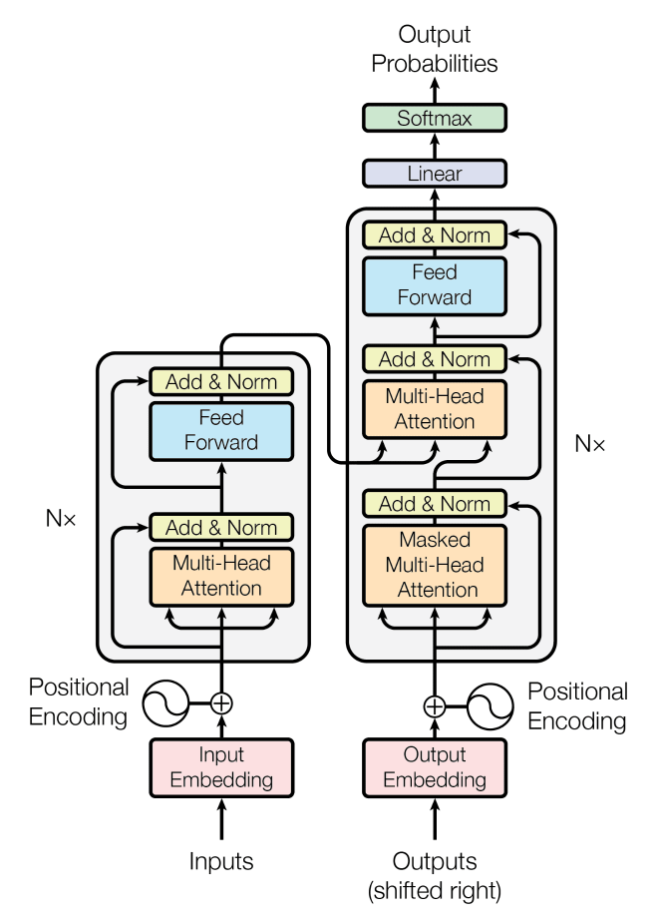
\includegraphics[width=0.5\textwidth]{figures/transformer.png}
		\caption{Transformer architecture. Left: Encoder. Right: Decoder.}
		\label{fig:transformer}
	\end{figure}
	
	In a nutshell, the task of the encoder, on the left half of the transformer architecture, is to map an input sequence to a sequence of continuous representations, which is then fed into a decoder. 
	The decoder, on the right half of the architecture, receives the output of the encoder together with the decoder output at the previous time step to generate an output sequence.
}

\Que{What is the purpose and working principle of the transformer encoder?}
\Ans{
	The transformer encoder encodes the input sequence into a set of continuous representations that capture contextual information. Each encoder layer refines these representations using self-attention and feed-forward networks. The key idea is that each position in the input can attend to all other positions, enabling modeling of complex dependencies.
}

\Que{What is the purpose and working principle of the transformer decoder?}
\Ans{
	The transformer decoder generates output tokens autoregressively. At each time step, it uses masked self-attention to process previous outputs and cross-attention to incorporate encoder information. The mask ensures that predictions for position \( t \) only depend on positions \( \leq t \), preserving causality.
}

\Que{What is causality and how is it implemented in the context of transformer decoder?}
\Ans{
	Causality ensures that the prediction at time step \( t \) does not depend on future tokens \( x_{t+1}, x_{t+2}, \ldots \). In the transformer decoder, this is implemented using a causal mask in the attention mechanism, which sets the attention weights of future positions to \(-\infty\) before applying softmax:
	
	\begin{equation}
		\text{MaskedAttention}(Q, K, V) = \text{softmax}\left(\frac{QK^\top}{\sqrt{d_k}} + M\right)V,
	\end{equation}
	where \( M_{i,j} = -\infty \) for \( j > i \), and 0 otherwise.
}

\Que{What are the advantages of transformers over other neural network architectures?}
\Ans{
	Transformers offer several key advantages:
	\begin{itemize}
		\item \textbf{Parallelism}: Unlike RNNs, all positions in the input can be processed simultaneously.
		\item \textbf{Global context}: Self-attention allows each token to access the full sequence context.
		\item \textbf{Scalability}: Easy to scale with data and model size (as seen in GPT, BERT).
		\item \textbf{Flexibility}: Effective in a wide range of domains beyond NLP (e.g., vision, protein folding).
	\end{itemize}
}

\Que{What is speech anticipation in conversation analogous to from the transformer architecture?}
\Ans{
	In human conversation, listeners often anticipate what will be said next. This is analogous to causal language modeling in transformers, where the model predicts the next token given previous ones. It reflects the same principle: using past context to make informed predictions about the future.
}

\Que{What is the vision transformer and how does it work?}
\Ans{
	The vision transformer (VIT) applies the transformer architecture to image classification. An image is divided into fixed-size patches (e.g., \(16 \times 16\) pixels), each flattened and linearly embedded. These embeddings, plus positional encodings, are passed through a standard transformer encoder.
	
	Unlike CNNs, VIT does not assume locality or translation invariance. It relies entirely on self-attention to model relationships across image patches.
}

\section{Natural language processing}

\Que{What is the goal in natural language processing?}
\Ans{
	The goal of natural language processing (NLP) is to design systems that can understand, interpret, generate, and interact with human language in a meaningful way. This includes tasks such as machine translation, sentiment analysis, question answering, and summarization. At its core, NLP involves mapping unstructured textual input into structured, meaningful representations that a machine can work with.
}

\Que{Which are the two philosophies of language modeling?}
\Ans{
	Language modeling can be approached through two main paradigms: Generative and discriminative modeling. Both aim to understand and process natural language, but differ fundamentally in what they model and how they are used.
	
	\begin{itemize}
		\item \textbf{Generative models}: These models learn the joint probability distribution over a sequence of tokens $
			p(x_1, x_2, \dots, x_T)$, 
		where \( x_t \in \mathcal{V} \) is the token at time step \( t \), and \( \mathcal{V} \) is the vocabulary. A common modeling assumption is that the joint probability factorizes using the chain rule as
		\begin{equation}
			p(x_1, \dots, x_T) = \prod_{t=1}^{T} p(x_t \mid x_1, \dots, x_{t-1}).
		\end{equation}
		That is, the probability of a token depends on all the previous tokens. These models are hence autoregressive and are trained to predict the next token given a context. Examples include GPT (generative pretrained transformer), traditional n-gram language models and RNN-based language models.
		
		\item \textbf{Discriminative models}: These models learn conditional probabilities, typically for classification tasks. Rather than modeling how likely a sequence is, they learn the probability of a label or missing token given the rest of the sequence as
		\begin{equation}
			p(y \mid x), \quad \text{or} \quad p(x_i \mid x_{\setminus i}),
		\end{equation} where \( x \) is an input sequence, \( y \) is a label (e.g., sentiment, topic) and \( x_{\setminus i} \) denotes the input with a token at position \( i \) masked out.
		\end{itemize}
		Discriminative models focus on understanding and classification, not generation. A major example is BERT (bidirectional encoder representations from transformers).
	
	In summary, generative models model the whole data distribution and are used to produce text, while discriminative models learn relationships between parts of data and are used for tasks like classification and inference.
}

\Que{What is tokenization in the context of natural language processing (NLP)?}
\Ans{
	Tokenization is the process of breaking raw text into smaller units called tokens, which serve as the atomic elements for further processing. Tokens can be words, subwords, or characters. This step is crucial for converting unstructured text into a structured format that can be embedded and processed by a neural network.
}

\Que{What ways to represent words numerically are there and how do they work and what are the advantages and disadvantages?}
\Ans{
	Several numerical word representations exist:
	
	\begin{itemize}
		\item \textbf{One-hot vectors}: Each word is assigned a unique index and represented as a binary vector. Simple, but does not capture similarity between words.
		\item \textbf{Co-occurrence vectors}: Based on how often words appear together in a context window. Large and sparse.
		\item \textbf{Word embeddings}: Dense, low-dimensional vectors trained to capture semantic relationships. Efficient and meaningful.
	\end{itemize}
	
	Word embeddings are widely used due to their ability to capture similarity and analogies; e.g. \texttt{king} - \texttt{man} + \texttt{woman} \(\approx\) \texttt{queen}.
}

\Que{What is the continuous bag of words (CBoW) word embedding algorithm and what are its interesting properties?}
\Ans{
	The continuous bag of words (CBoW) model predicts a target word from surrounding context words. Given context words \( \{x_{t-n}, \dots, x_{t+n} \setminus x_t\} \), the model predicts \( x_t \). The input is the average of the embeddings of context words. 
	
	The CBoW model has a few interesting properties, namely that it is efficient to train on large corpora, produces high-quality embeddings and encodes semantics via context, capturing word similarity.
}

\Que{What is the co-occurrence matrix in the context of natural language processing?}
\Ans{
	A co-occurrence matrix records how often words occur together within a defined context window in a large corpus. Rows and columns represent vocabulary terms, and the \( (i,j) \)-th entry is the count of times word \( j \) appears in the context of word \( i \). This matrix captures distributional information that can be used to compute word similarity or serve as input to dimensionality reduction techniques like singular value decomposition (SVD).
	
Consider the following example sentence ``The cat sits on the mat. The dog sits nearby.''
	With a context window of size 1 (one word before and after), and a vocabulary
	\[
	\text{Vocab} = [\texttt{the}, \texttt{cat}, \texttt{sits}, \texttt{on}, \texttt{mat}, \texttt{dog}, \texttt{nearby}],
	\]
	we can construct a symmetric co-occurrence matrix where each entry \( C_{ij} \) counts how often word \( j \) appears next to word \( i \):
	\[
	\begin{array}{c|ccccccc}
		& \texttt{the} & \texttt{cat} & \texttt{sits} & \texttt{on} & \texttt{mat} & \texttt{dog} & \texttt{nearby} \\
		\hline
		\texttt{the} & 0 & 1 & 0 & 0 & 1 & 1 & 0 \\
		\texttt{cat} & 1 & 0 & 1 & 0 & 0 & 0 & 0 \\
		\texttt{sits} & 0 & 1 & 0 & 1 & 0 & 1 & 0 \\
		\texttt{on} & 0 & 0 & 1 & 0 & 1 & 0 & 0 \\
		\texttt{mat} & 1 & 0 & 0 & 1 & 0 & 0 & 0 \\
		\texttt{dog} & 1 & 0 & 1 & 0 & 0 & 0 & 1 \\
		\texttt{nearby} & 0 & 0 & 0 & 0 & 0 & 1 & 0 \\
	\end{array}.
	\]
	This matrix captures how words are distributed around one another. For example, the word \texttt{sits} appears next to \texttt{cat}, \texttt{dog}, and \texttt{on}, reflected in its corresponding row.
	
If two words have similar co-occurrence patterns (e.g., \texttt{cat} and \texttt{dog}), they are likely to have similar meanings — a principle known as the \textit{distributional hypothesis}.
}

\Que{How does singular value decomposition (SVD) for any matrix \( X \) work? Why is it useful in many applications, e.g. with the co-occurrence matrix?}
\Ans{
	Singular Value Decomposition (SVD) factorizes any real matrix \( X \in \mathbb{R}^{m \times n} \) as
	
	\begin{equation}
		X = U \Sigma V^\top,
	\end{equation}
	where \( U \in \mathbb{R}^{m \times m} \) and \( V \in \mathbb{R}^{n \times n} \) are orthogonal matrices containing the left and right singular vectors, respectively, and \( \Sigma \in \mathbb{R}^{m \times n} \) is a diagonal matrix with non-negative singular values \( \sigma_1 \geq \sigma_2 \geq \dots \geq 0 \) on the diagonal. This decomposition is useful for dimensionality reduction, especially in natural language processing.
	
	In the context of NLP, applying SVD to a word co-occurrence matrix allows us to discover latent semantic dimensions. Each word is represented by a dense vector whose structure reflects global statistical patterns in the corpus. Truncating the decomposition to the top \( k \) singular values and vectors yields a rank-\( k \) approximation of the original matrix, preserving the most significant directions in the data while reducing noise and dimensionality. Reducing dimensionality in the co-occurrence matrix is necessary because it is sparse.
	
	SVD is closely related to Principal Component Analysis (PCA). Given a mean-centered data matrix \( X \in \mathbb{R}^{n \times d} \), PCA performs an eigen-decomposition on the covariance matrix
	\begin{equation}
		C = \frac{1}{n-1} X^\top X.
	\end{equation}
	The eigenvectors \( v_i \) of \( C \) define the principal directions, and the corresponding eigenvalues \( \lambda_i \) indicate how much variance is explained by each direction:
	\begin{equation}
		C v_i = \lambda_i v_i.
	\end{equation}
	However, rather than computing this directly, PCA is typically implemented via the SVD of \( X \). From the SVD \( X = U \Sigma V^\top \), it follows that
	\begin{equation}
		X^\top X = V \Sigma^2 V^\top,
	\end{equation}
	so the eigenvalues of \( X^\top X \) are \( \lambda_i = \sigma_i^2 \), and the eigenvectors are the columns of \( V \). Thus, the eigenvalues obtained in PCA are equal to the squares of the singular values obtained in SVD.
}

\Que{What is GloVe, how does it work and what are advantages and disadvantages?}
\Ans{
	Global vectors for word representation (GloVe) is a word embedding algorithm that learns vector representations of words by leveraging global co-occurrence statistics from a large corpus. 
	The model minimizes a weighted least squares objective:
	\begin{equation}
		J = \sum_{i,j=1}^V f(X_{ij})\left(w_i^\top \tilde{w}_j + b_i + \tilde{b}_j - \log X_{ij}\right)^2,
	\end{equation}
where \( V \) is the vocabulary size, \( X_{ij} \) is the number of times word \( j \) appears in the context of word \( i \),  \( w_i \in \mathbb{R}^d \) is the word vector for word \( i \) (target embedding), \( \tilde{w}_j \in \mathbb{R}^d \) is the context word vector for word \( j \), \( b_i \) and \( \tilde{b}_j \) are bias terms associated with word \( i \) and context word \( j \), respectively and \( f(X_{ij}) \) is a weighting function that reduces the influence of extremely frequent or infrequent co-occurrences.
	
	The objective ensures that the inner product \( w_i^\top \tilde{w}_j \), adjusted by biases, approximates \( \log X_{ij} \), which reflects how strongly word \( j \) is associated with word \( i \) in the corpus. A major advantage of GloVe is that it is efficient and scalable for large corpora and produces high-quality embeddings that reflect semantic relationships. A major disadvantage of GloVe is that each word has a single embedding vector. This means that the model is unable to handle multiple meanings of a word depending on context.
}


\section{Representation learning}

\Que{What is representation learning and what is the goal in this kind of artificial intelligence?}
\Ans{
	Representation learning refers to the process of automatically discovering meaningful features or representations of the input data that make it easier to perform downstream tasks such as classification or regression. The goal is to transform raw data into useful representations that capture the underlying factors of variation, often in a lower-dimensional or more structured space.
}

\Que{What are applications of representation learning?}
\Ans{
	Representation learning has wide applications, as it is used as a preprocessor to find meaningful features for many tasks, including the following:
	\begin{itemize}
		\item Image classification and object detection.
		\item Speech recognition.
		\item Natural language processing (e.g. embeddings).
		\item Recommender systems.
		\item Robotics (e.g. sensor fusion and control).
		\item Healthcare (e.g. patient embeddings for diagnostics).
	\end{itemize}
}

\Que{What is the idea behind transfer learning?}
\Ans{
	Transfer learning is the idea of using a model trained on one task or domain and adapting it to a new, related task. This is done by transferring the learned representations (e.g. features or weights) and fine-tuning them on the target task. This approach is especially powerful when labeled data in the target domain is scarce.
}

\Que{What is transfer learning via fine-tuning and how does it work; how can it be visualized?}
\Ans{
	Transfer learning via fine-tuning involves taking a model that was pre-trained on a large dataset and task (e.g. ImageNet for image classification) and adapting it to a new, possibly smaller dataset and related task. This is done by initializing the new model with the pre-trained weights and continuing training (fine-tuning) on the new task. 
	
	As an example imagine a model trained to classify animals. For a new task, such as classifying bird species, we reuse the layers that already detect edges, textures, and shapes, and fine-tune the final layers to distinguish between bird species. See also \cref{fig:fine-tuning} for a visualization of how transfer learning via fine-tuning is.
	\begin{figure}[h]
		\centering
		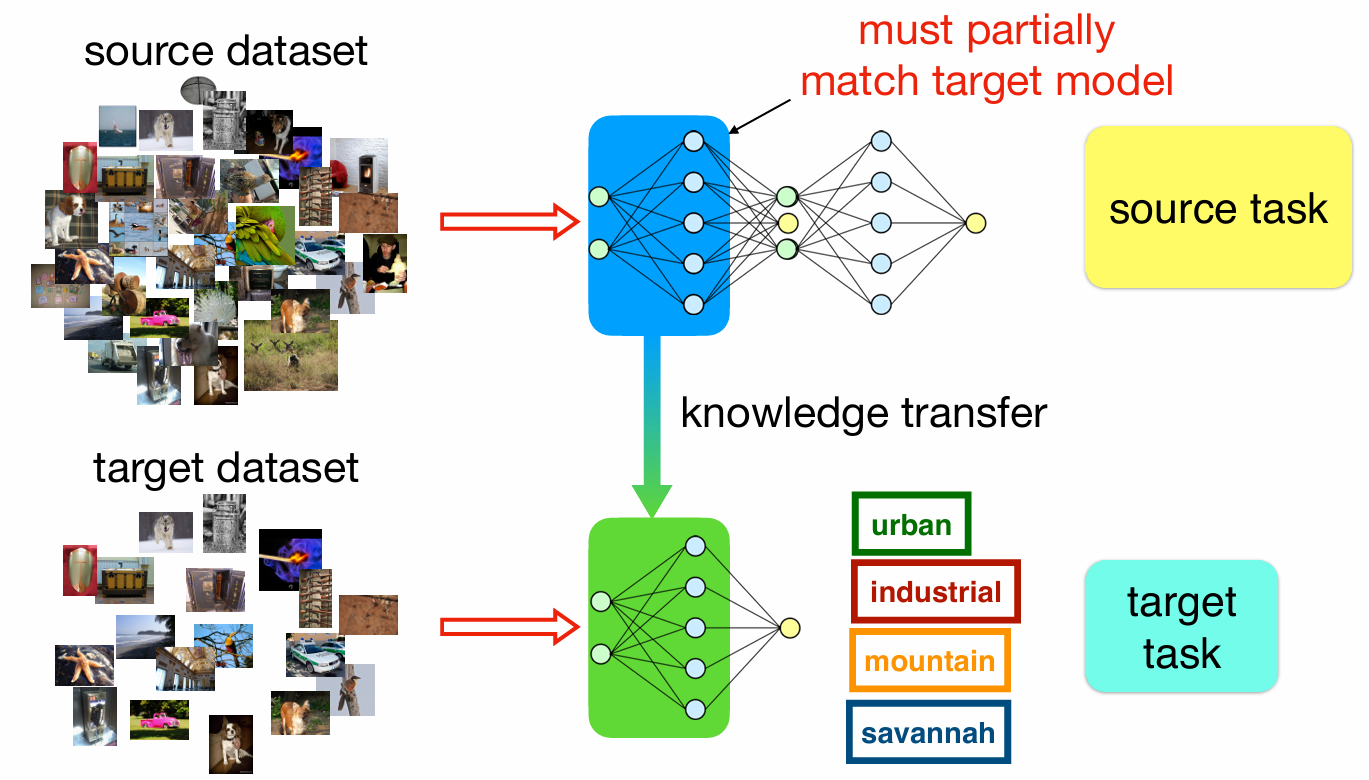
\includegraphics[width=0.5\textwidth]{figures/fine-tuning.png}
		\caption{Transfer learning via fine-tuning.}
		\label{fig:fine-tuning}
	\end{figure}
}

\Que{What is the idea behind domain adaptation?}
\Ans{
	Domain adaptation is a subfield of transfer learning where the source and target tasks are the same, but the domains differ (e.g. sentiment analysis on product reviews vs. tweets). The goal is to learn representations that are invariant across domains to ensure good generalization to the target domain.
}

\Que{What is the idea behind one-shot learning?}
\Ans{
	One-shot learning aims to generalize from a single or very few labeled examples per class. This is achieved by learning a feature space where similar inputs are close together, often using metric learning techniques or pre-trained embeddings combined with nearest-neighbor classification.
	
	One-shot learning is somehow related to semi-supervised learning: One-shot learning is like teaching someone to recognize a new animal from just one picture. Semi-supervised learning however is like giving someone a few labeled examples and a lot of unlabeled images and letting them infer the rest by pattern matching.
}

\Que{What is the idea behind zero-shot learning?}
\Ans{
	Zero-shot learning refers to the ability to recognize and classify categories that the model has never seen during training. This is typically achieved by learning representations in a shared space (e.g. text and images) and using semantic information (like class descriptions) to generalize to unseen classes.
}

\Que{What is CLIP and how can it be used for inference?}
\Ans{
	Contrastive language-image pretraining (CLIP) is a model that jointly learns embeddings for text and images using a contrastive loss. The model is trained to bring together embeddings of matching image-caption pairs and push apart mismatched pairs.
	
	For inference, given an image and a set of textual descriptions (labels), CLIP computes similarity scores between the image embedding and each text embedding. The label with the highest similarity score is selected, enabling zero-shot classification.
}

\Que{What is an embedding in the context of deep learning?}
\Ans{
	In deep learning, an embedding refers to a mapping from a high-dimensional, often discrete input space (such as words, items, or entities) into a continuous, dense, low-dimensional vector space. This transformation allows the model to represent symbolic or categorical data in a form suitable for numerical computation and learning.
	
	Formally, let \( \mathcal{V} \) denote a discrete vocabulary (e.g. of size \( |\mathcal{V}| \)), and let each token \( x \in \mathcal{V} \) be represented as a one-hot vector \( e_x \in \mathbb{R}^{|\mathcal{V}|} \). An embedding layer is then a matrix \( E \in \mathbb{R}^{|\mathcal{V}| \times d} \), where \( d \ll |\mathcal{V}| \) is the embedding dimension. The embedding of token \( x \) is given by
	\begin{equation}
		\text{Embed}(x) = E^\top e_x = E_{x} \in \mathbb{R}^d.
	\end{equation}
	That is, embedding \( x \) means selecting the \( x \)-th row of the matrix \( E \). Each row of \( E \) corresponds to a dense vector representation of a token in the vocabulary.
	
	Embeddings are central in tasks involving discrete input, such that they can be processed by units of deep learning such as feedforward networks or other types of networks. Well-trained embeddings capture semantic or structural similarity: Similar inputs are mapped to nearby points in the embedding space. For instance, in word embeddings, the vectors for \texttt{king}, \texttt{queen}, \texttt{man}, and \texttt{woman} may satisfy relationships like
	\[
	\text{Embed}(\texttt{king}) - \text{Embed}(\texttt{man}) + \text{Embed}(\texttt{woman}) \approx \text{Embed}(\texttt{queen}).
	\]
}


\Que{What is the difference between local and distributed representation?}
\Ans{
	In a local representation, each concept or category is represented by the activation of a single neuron or dimension. For example, imagine a neural network with 10 output neurons where neuron 3 fires only when recognizing a ``cat'', and no other neuron activates. This is a one-to-one mapping: each neuron corresponds to exactly one concept. Such representations are simple but not very flexible or robust.
	
	In a distributed representation, a concept is represented by a pattern of activations across multiple neurons. For example, a ``cat'' might be represented by neurons 2, 4, and 7 being active simultaneously. Importantly, these same neurons may also participate in representing other concepts like ``dog'' or ``tiger'', but with different activation patterns. This makes distributed representations more compact, expressive, and capable of generalizing to unseen combinations.
}

\section{Self-supervised learning}

\Que{What is self-supervised learning about and what is the main goal?}
\Ans{
	Self-supervised learning is a machine learning paradigm where the model learns to predict parts of the input from other parts, effectively creating its own labels from raw data. The main goal is to learn useful and generalizable feature representations without requiring human-annotated labels. This is especially valuable when labeled data is scarce or expensive to obtain.
}

\Que{What is the difference between self-supervised learning, supervised learning and unsupervised learning?}
\Ans{These types of AI-learning are characterized by the following properties:
	\begin{itemize}
		\item \textbf{Supervised Learning:} Uses labeled data \((x, y)\) to learn a mapping \(f(x) \rightarrow y\). Models a probability distribution $p(y|x)$ of labels $y$ given input data $x$.
		\item \textbf{Unsupervised Learning:} Finds patterns in unlabeled data $x$, such as clustering or dimensionality reduction. Models a probability distribution $p(x)$ of the input data.
		\item \textbf{Self-supervised Learning:} Constructs pseudo-labels $\hat{y}$ from the input data $x$ itself to train in a supervised-like manner, often serving as a pre-training strategy for other tasks. Models a probability distribution $p(\hat{y}|x)$ of pseudo-labels $\hat{y}$ given input data $x$.
	\end{itemize}
}

\section{Autoencoders and variational autoencoders}

\Que{How can the general principle of an autoencoder be stated in few words and an illusration?}
\Ans{
	An autoencoder is a neural network that learns to compress input data into a lower-dimensional representation (encoding) and then reconstruct it back (decoding). 
	
Illustratively and mathematically, this can be expressed with the formula
	\begin{equation} x \rightarrow \text{Encoder } f(x) = z \rightarrow \text{Decoder } g(z) = \hat{x} \end{equation}
	where the goal is \( \hat{x} \approx x \).
}

\Que{Which function does the autoencoder try to ``build''?}
\Ans{
	The autoencoder tries to learn the identity function \( x \mapsto \hat{x} \approx x \), but only via a low-dimensional latent representation \( z = f(x) \), enforcing useful feature extraction rather than direct copying. That is, the autoencoder consists of an encoder $f(x)$  and a decoder $g(z)$. The learned function $\text{Id}(x) \approx x$ is then given by \begin{equation}
		\text{Id}(x) = g(f(x)) = g \circ f(x).
	\end{equation}
}

\Que{What are the probabalistic mathematics used under the hood of autoencoders?}
\Ans{
	Autoencoders can be extended into a probabilistic framework, notably as variational autoencoders (VAEs), which model the generative process of the data using latent variables.
	
	We assume that data \( x \in \mathbb{R}^n \) is generated from a latent variable \( z \in \mathbb{R}^k \) through a two-step process
	\begin{equation}
		z \sim p(z), \quad x \sim p(x|z),
	\end{equation}
	where \( p(z) \) is typically chosen as a standard normal distribution \( \mathcal{N}(0, I) \), and \( p(x|z) \) is the likelihood or decoder distribution parameterized by a neural network.
	We aim to maximize the marginal log-likelihood
	\begin{equation}
		\log [p(x)] = \log \left[\int p(x, z) \, \mathrm{d}z\right]
	\end{equation}
	of the data. Since this integral is intractable for complex models, we introduce a variational approximation \( q(z|x) \) to the true posterior \( p(z|x) \). Now consider
	\begin{equation}
		\log [p(x)] = \log \left[\int \frac{q(z|x)}{q(z|x)} p(x, z) \, \mathrm{d}z\right].
	\end{equation}
	Multiplying and dividing by \( q(z|x) \), we apply Jensen's inequality (since \( \log \mathbb{E}[\cdot] \geq \mathbb{E}[\log(\cdot)] \)) as
	\begin{equation}
		\log [p(x)] \geq \mathbb{E}_{q(z|x)} \left[ \log \frac{p(x, z)}{q(z|x)} \right].
	\end{equation}
	We define this lower bound as the ELBO
	\begin{equation}
		\mathcal{L}_{\text{ELBO}}(x) := \mathbb{E}_{q(z|x)} \left[ \log p(x, z) - \log q(z|x) \right].
	\end{equation}
	Since \( p(x, z) = p(x|z) p(z) \), this becomes
	\begin{equation}
		\mathcal{L}_{\text{ELBO}}(x) = \mathbb{E}_{q(z|x)}[\log p(x|z)] - \mathrm{KL}(q(z|x) \| p(z)).
	\end{equation}
	
	The first term in the ELBO is the expected log-likelihood (or reconstruction term), which ensures that \( x \) can be reconstructed from \( z \). The second term is the Kullback-Leibler divergence between the approximate posterior \( q(z|x) \) and the prior \( p(z) \), acting as a regularizer. In practice, both \( q(z|x) \) and \( p(x|z) \) are implemented as neural networks, and training is performed by maximizing the ELBO across the dataset.
}



\Que{What can be done to avoid the trivial identity in autoencoder training?}
\Ans{In order to avoid that a autoencoder learns a trivial identity, one can undertake one of the following strategies:
	\begin{itemize}
		\item Use a bottleneck: Restrict the latent space to fewer dimensions than the input. This ensures that the encoder must learn to compress the input dimension such that meaningful features are extracted to the latent space.
		\item Add noise to the input (e.g. denoising autoencoder).
		\item Add regularization (e.g. sparsity or Kullback-Leibler divergence as in VAEs).
	\end{itemize}
}

\Que{What is the principle of denoising autoencoders? Why are these types of autoencoders currently the ``golden standard'' of generative AI?}
\Ans{
	Denoising autoencoders are trained to reconstruct clean inputs from corrupted versions. This encourages the model to learn robust and generalizable features.
	
	They form the basis for generative models like diffusion models, where the generation process involves denoising from noise, making them foundational to state-of-the-art generative AI.
}

\Que{How does a variational autoencoder work?}
\Ans{
	A variational autoencoder learns a probabilistic latent variable model by jointly learning an encoder \( q(z|x) \) that approximates the posterior, a decoder \( p(x|z) \) that reconstructs data and a prior \( p(z) \), typically \( \mathcal{N}(0, I) \).
	
	The objective is to maximize the ELBO (see derivation above) $
	\mathcal{L}_{\text{VAE}} = \mathbb{E}_{q(z|x)}[\log p(x|z)] - \text{KL}(q(z|x) \| p(z)),$
	whis enables sampling new data by sampling \( z \sim p(z) \) and generating \( x \sim p(x|z) \).
}

\Que{What is a masked autoencoder and how does it work?}
\Ans{
	A masked autoencoder (MAE) is a self-supervised learning method where a large portion of input (e.g., image patches or tokens) is masked, and the model is trained to reconstruct the missing content.
	
	The encoder processes only the unmasked patches, and a lightweight decoder attempts to reconstruct the full input from the encoded partial view. This encourages the model to learn meaningful representations even with limited visible context.
}

\section{Generative methods}

\Que{What is the general idea of generative modeling?}
\Ans{
	Generative modeling involves learning the data distribution \( p(x) \) so that we can sample new data points that resemble the training data. This includes approaches like VAEs, GANs, normalizing flows, and diffusion models.
}

\Que{What is the working principle of generative adversarial networks (GAN)? How is it trained?}
\Ans{
	A GAN consists of two neural networks:
	\begin{itemize}
		\item The \textbf{Generator} \( G(z) \): It maps random noise \( z \) to fake data \( x' \).
		\item The \textbf{Discriminator} \( D(x) \): It tries to distinguish real data from generated data.
	\end{itemize}
	Both are trained in a minimax game-theoretical manner, namely
	\begin{equation}
	\min_G \max_D \left(\mathbb{E}_{x \sim p_{\text{data}}}[\log D(x)] + \mathbb{E}_{z \sim p(z)}[\log(1 - D(G(z)))]\right).
	\end{equation}
	
	Training a GAN consists of alternating between alternates between:
	\begin{enumerate}
		\item updating the discriminator to better separate real and fake samples
		\item and updating the generator to fool the discriminator.
	\end{enumerate}
	This iterative process continues until the generator produces data that is indistinguishable from real data.
}

\Que{What is the basic principle of normalizing flows?}
\Ans{
	Normalizing flows learn an invertible mapping \( f \) between a simple distribution \( p(z) \) and the data distribution \( p(x) \), enabling exact likelihood computation via the change of variables formula:
	\[
	p(x) = p(z) \left| \det \left( \frac{\partial f^{-1}}{\partial x} \right) \right|
	\]
	where \( z = f^{-1}(x) \).
}

\Que{How are normalizing flows trained?}
\Ans{
	They are trained by maximizing the exact log-likelihood of the data using the change-of-variables formula. Each step in the flow must be invertible and have a tractable Jacobian determinant.
}

\Que{What is the basic principle of diffusion models?}
\Ans{
	Diffusion models generate data by learning to reverse a Markov process that gradually adds noise to data until it becomes pure noise. The model learns to denoise step-by-step, effectively reversing this diffusion process.
}

\Que{How are diffusion models trained?}
\Ans{
	They are trained to predict the noise added at each step of the forward diffusion process using a loss such as mean squared error between predicted and actual noise. The network learns to denoise data through thousands of iterative steps, starting from Gaussian noise.
}


\section{Exam 2024}
\subsection{Original questions}
% see mock exams
\Que{Indicate whether the following statements are true or false:
\begin{enumerate}
	\item The purpose of adding activation functions to neural networks is to reduce overfitting.
	\item During training with stochastic gradient descent, the learning rate is set low to avoid underfitting.
	\item Dropout leads to sparsity in the trained weights.
	\item Batch normalization is a non-linear transformation to center the whole dataset around the origin.
	\item Weight initialization does not affect the performance of a neural network.
	\item L1-regularization adds the sum of the absolute values of the weights to the loss function to penalize large weights.
	\item In a fully connected neural network, each neuron in one layer is connected to every neuron in the next layer.
	\end{enumerate}}
\Ans{ Here are the justified answers:
	\begin{enumerate}
		\item False: Activation functions introduce non-linearity, not regularization.
		\item False: A low learning rate risks underfitting, not avoids it.
		\item False: Dropout causes neuron deactivation, not weight sparsity.
		\item False: Batch norm is linear and applied per batch, not the full dataset.
		\item False: Poor initialization affects training stability.
		\item True: L1-regularization penalizes large weights $\theta$ via an additional term $\lambda \|\theta\|$ in the loss function.
		\item True: Full connectivity implies every neuron connects to the next layer.
\end{enumerate}}

\Que{Gradient descent is used for optimization. Given a loss function $L(x)$, an initial value $x_0$, gradient descent evolves according to $x_{t+1} = x_t - \alpha\nabla L(x_t)$ for $t=0,1,\dots$. Compute gradient descent for the cases below and determine convergence!
\begin{enumerate}
	\item $L(x) = |x|$ for $x_0=1$ and $\alpha=2$.
	\item $L(x) = x^2$ for $x_0 = 1$ and $\alpha= 1$.
	\end{enumerate}}
\Ans{ Here are the justified answers:
	\begin{enumerate}
	\item  Consider $L(x) = |x|$, $x_0 = 1$, $\alpha = 2$. The gradient is given by $	\nabla L(x) = \text{sign}(x)$, then we have $x_1 = 1 - 2 \cdot 1 = -1 $ and $x_2 = -1 - 2(-1) = 1$. We can thus see that we have an oscillation between $-1$ and $1$, therefore gradient descent diverges. 
	\item  We have $L(x) = x^2$, $x_0 = 1$, $\alpha = 1$. Now, the gradient gives $\nabla L(x) = 2x$ with 
		$x_1 = 1 - 1 \cdot 2 = -1$ and $ x_2 = -1 + 2 = 1 $. Again, we have an oscillation, hence the algorithm diverges.
\end{enumerate}}

\Que{Which of the following would you consider to be valid activation functions
	(elementwise non-linear) to train a neural net in practice?
	\begin{enumerate}
		\item $f(x) = -\min(0,x)$.
		\item $f(x) = 0.1x + 1$.
		\item $f(x) = \begin{cases}
			\min(0.5x,x), & x \geq 0 \\
			\min(0.5x,x), & x < 0
		\end{cases}.$
		\item $f(x) = \begin{cases}
			\min(0,x), & x \geq 0 \\
			\min(0.5x,x), & x < 0
		\end{cases}.$
		\end{enumerate}}
\Ans{here are the justified answers:
	\begin{enumerate}
	\item  Valid (non-linear).
	\item  Invalid (linear).
	\item  Invalid (linear across domain).
	\item  Valid (non-linear branching).
	\end{enumerate}
}

\Que{Consider the recurrent model $h_t = Ah_{t-1} + Bx_t$ and $y_t = Ch_t$, where $x_t$, $h_t$, $y_t$ are in $\mathbb{R}^d$ and are the input, the hidden state and the output at time $t$. $A$, $B$, and $C$ are $d\times d$ matrices. Answer the following questions:
\begin{enumerate}
	\item Could one build a powerful deep recurrent neural network by using only a
	sequence of models like the one above?
	\item Show that the output sequence $(y_0,...,y_t)$ can be obtained as a product of
	the inputs $(x_0,...,x_t)$ with some matrices $(K_0,...,K_t)$. That is, $y_s = \sum_{i \leq s} K_{s-i} x_i$,
	where $K_i$ are $d \times d$ matrices that depend on $A$,$B$, and $C$. Show all steps and provide
	the explicit expression for $K_i$.
	\item Can teacher forcing be applied to the encoder to ease the training? Can it be
	applied to the decoder?
	\item Do you expect the model to benefit from replacing the encoder with a bidi
	rectional RNN?
	\end{enumerate}
}

\Ans{Below the answers:
\begin{enumerate}
	\item No, there is no nonlinearity in the network design.
	\item We are given a linear recurrent neural network model defined as:
	\begin{align*}
		h_t &= A h_{t-1} + B x_t,  \\
		y_t &= C h_t.
	\end{align*}
	where \( x_t, h_t, y_t \in \mathbb{R}^d \), and \( A, B, C \in \mathbb{R}^{d \times d} \). We express \( h_t \) as a function of the inputs \( x_0, x_1, \ldots, x_t \):
	\begin{align*}
		h_0 &= B x_0 \\
		h_1 &= A h_0 + B x_1 = A B x_0 + B x_1 \\
		h_2 &= A h_1 + B x_2 = A^2 B x_0 + A B x_1 + B x_2 \\
		&\vdots \\
		h_t &= A^t B x_0 + A^{t-1} B x_1 + \cdots + A B x_{t-1} + B x_t \\
		&= \sum_{i=0}^{t} A^{t - i} B x_i.
	\end{align*}	
	Substituting the expression for \( h_t \) into the previous equation we get
	\begin{align*}
		y_t &= C h_t = C \sum_{i=0}^{t} A^{t - i} B x_i \\
		&= \sum_{i=0}^{t} C A^{t - i} B x_i.
	\end{align*}	
	We want to express the output as
	\[
	y_s = \sum_{i=0}^{s} K_{s - i} x_i.
	\]
	Comparing terms, we identify
	\[
	K_{s - i} = C A^{s - i} B
	\]
	and hence
	\[
	y_s = \sum_{i=0}^{s} C A^{s - i} B x_i
	\quad \text{with} \quad
	K_{s - i} = C A^{s - i} B.
	\]
	\item No. The encoder does not have an output for each input. For the decoder however the answer is yes, because it uses previous output.
	\item Yes. The encoder can scan the sequence in both directions and obtain a
	richer representation of the sequence. 
	\end{enumerate}
}

\Que{Given the query $Q \in \mathbb{R}^{n\times d_k}$, the key $K \in \mathbb{R}^{n\times d_k}$ and the value $V \in \mathbb{R}^{n\times d_k}$, aswell as the scaled dot-product calculates as \begin{equation}
		\text{Attention}(Q,K,V) = \text{Softmax}\left(\frac{QK^\top}{\sqrt{d_k}}\right)V.
	\end{equation} Answer the following questions:
\begin{enumerate}
	\item How are $Q$, $K$, and $V$ obtained from the input sequence $x \in \mathbb{R}^{n\times d}$ in a typical implementation?
	\item What is the role of the scaling factor $d_k$?
	\item Which of the masks defines causal attention (i.e. a query token in the sequence can only cay attention to past key tokens)?
	\begin{enumerate}
		\item $M_{ij} = 1$, $j\leq i$, $M_{ij} = 0$, $j > i$.
		\item $M_{ij} = 1$, $j \leq i$, $M_{ij} = -\infty$, $j > i$.
		\item $M_{ij} = 1$, $i=j$, $M_{ij} = -\infty$, $i \neq j$.
		\item $M_{ij} = 1$, $|i-j| < 5$, $M_{ij} = 0$, $|i-j| \geq 5$.
	\end{enumerate}
	\item What is the purpose of position encoding in transformers? Describe two different types of position encodings!
	\end{enumerate}}
\Ans{The answers are the following:
\begin{enumerate}
	\item All the matrices are different linear projections of the input.
	\item The factor $d_k$ prevents the values in $QK^\top$ from getting too large. If the values in $QK^\top$ get too large, it can push the softmax into regions with small gradients and thereby mitigate training efficiency. In some cases it is useful to restrict the attention to a subset of tokens, which can be achieved via a masking mechanism.
	\item No, Yes, No, No.
	\item Without position encodings the tokens do not know their relative position with respect to other tokens in the sequence. Hence, they are treated as bag of words, which can diminish performance. Examples are sine and cosine encodings or learned encodings.
	\end{enumerate}}

\Que{utoencoders (AE) are models that aim to learn an efficient representation of the data, typically for dimensionality reduction. Principal component analysis (PCA) is also used for
	the same purpose. Explain the reasoning in all of the following questions:
	\begin{enumerate}
		\item What is the main difference between the two approaches AE and PCA?
		\item Which approach is more interpretable?
		\item I what cases is it preperable to use PCA?
		\end{enumerate}}
\Ans{The answers are as follows:
	\begin{enumerate}
		\item Unlike PCA, AE's can learn complex, non-linear mappings due to the non-linear activation functions in their neural network layers. This makes them suitable for data that live in a non-linear space.
		\item However, the learned latent representations in AE's are typically less interpretable compared to PCA's principal components. They do not have a straightforward relationship to the original features.
		\item AE's generally require more computational resources and longer training times compared to PCA. Thus, PCA is preferable when the data is inherently linear, and interpretability and computational efficiency are important.
	\end{enumerate}
}

\Que{There are three identified fundamental factors to characterize generative
	learning methods (also referred to as the trilemma). Explain the differences between
	VAEs, Generative generative adversarial networks (GANs), and denoising diffusion models (DDM) in
	terms of these three factors.}
\Ans{
Current generative learning frameworks cannot yet simultaneously satisfy all three key requirements:
\begin{enumerate}
	\item high-quality sampling,
	\item mode coverage and sample diversity,
	\item fast and computationally inexpensive sampling.
\end{enumerate}
VAE's satisfy (ii) and (iii), GAN's satisfy (i) and (iii), and DDM's satisfy (i) and (ii).}

\Que{VAEs are usually constructed so that their latent vectors have a Gaussian distribution. To train a model we use the reparameterization trick for the Gaussian distribution: sampling $x$ from $\mathcal{N}(\mu, \sigma^2)$ is equivalent to sampling $\varepsilon$ from $\mathcal{N}(0, 1)$ and then computing $x = \mu + \sigma \varepsilon$. Why do we need this trick?}
\Ans{We need it to compute the backpropagation. The reparameterization trick is a technique commonly used to enable gradient-based optimization over stochastic variables. We cannot calculate the gradient with respect to $x \sim \mathcal{N}(\mu, \sigma^2)$, but we can calculate it with respect to $\mu$ and $\sigma$ in the case of $x = \mu + \sigma \varepsilon$, where $\varepsilon \sim \mathcal{N}(0, 1)$.}

\Que{The reparameterization trick can be adapted to any distribution. The idea is to sample a random variable $U$ that is uniform in $[0, 1]$, and to map it to any desired random variable $Z \sim f(z)$. To do that, one needs to compute the Cumulative Distribution Function (CDF) $F(z)$ of $Z$ (it is the integral of $f(z)$ from $-\infty$ to $z$). Then, the random variable $\tilde{Z} = F^{-1}(U)$ has the same distribution as $Z$, where $F^{-1}(u)$ is the inverse of $F(z)$.
Apply the reparameterization trick in the case of the exponential distribution
\[
f(z) = 
\begin{cases}
	\lambda \exp(-\lambda z), & \text{if } z \geq 0, \\
	0, & \text{otherwise.}
\end{cases}
\]
\textit{Hint:} Eq. (7) is the probability density function, i.e., the derivative of the CDF $F(z)$ with respect to $z$. Then, the CDF of $Z$ is equal to $F(z) = 1 - \exp(-\lambda z)$.
}
\Ans{
Let’s find the inverse of this CDF. We have
\begin{align}
	u &= F_\lambda(z) = 1 - \exp(-\lambda z) \\
	1 - u &= \exp(-\lambda z) \\
	\log(1 - u) &= -\lambda z \\
	z &= -\frac{1}{\lambda} \log(1 - u).
\end{align} Thus, the random variable $Z \sim \text{Exp}(\lambda)$ has the same distribution as the random variable
\[
\tilde{Z} = F^{-1}_\lambda(U) = -\frac{1}{\lambda} \log(1 - U),
\]
where the random variable $U$ is uniform on $[0, 1]$. If $U$ is uniform on $[0, 1]$, then $\tilde{U} = 1 - U$ is also uniform on $[0, 1]$. So, to sample $z$ from $\text{Exp}(\lambda)$, we can:
\begin{enumerate}
	\item sample $\varepsilon$ from $U[0, 1]$ and
	\item compute $z = -\frac{1}{\lambda} \log \varepsilon$.
	\end{enumerate}}

\Que{We want to train a fully convolutional neural network (CNN) for binary image segmentation,
	where each input pixel is classified as foreground or background. The network consists of
	only 3 convolutional layers. During training, each image is resized to 256 × 256 × 3 pixels,
	where 256 × 256 is the input spatial dimensions and 3 the number of image channels.
	For each convolutional layer, we need to define the following hyper-parameters: the kernel
	size $k$, the number of input channels $c_{in}$, the number of output channels $c_{out}$, the stride $s$, and
	the padding $p$. We want to use fewer than 20 filters at each layer. Answer the following questions:
	\begin{enumerate}
		\item Determine the spatial dimensions of the network output corresponding to the training images.
		\item Suppose that the padding $p = 0$ for all the convolutional layers. Define the hyper-parameters of all the layers. If more than one choice is valid for a hyper-parameter, pick one of your choice.
		\item We choose $k = 1$ and $s = 1$ for all 3 layers and set the other hyper-parameters to satisfy the output dimension requirement. Explain why this is a suboptimal choice.
		\item After training the model, we find that one of the images in the test set has dimensions $128 \times 128 \times 3$. Would we get an error if we applied the model to this image? If yes, how can it be fixed? If no, why?
		\item We want to train a vanilla feed-forward network to solve the same segmentation task. Which network contains fewer parameters? Justify your answer.
		\end{enumerate}}
\Ans{
	The answers are as follows:
	\begin{enumerate}
		\item Given that the task to solve is image segmentation, the spatial dimensions of the output should match the spatial dimensions of the input, which is $256 \times 256$.
		\item The output shape of a convolutional layer can be calculated using the formula:
		\[
		\frac{N - k + 2p}{s} + 1,
		\]
		where $N$ is the input dimension. To achieve an output size that matches the input size, each layer must have the same input and output dimensions. Given that $p = 0$, we need $k = 1$ and $s = 1$ for all layers.
		\begin{itemize}
			\item For the first layer, set $c_{in} = 3$.
			\item For the last layer, $c_\text{out}$ can be either 1 or 2.
			\item $c_{in}$ of the second layer should equal $c_{out}$ of the first layer.
			\item $c_{in}$ of the third layer should equal $c_{out}$ of the second layer.
		\end{itemize}
		\item Using $k = 1$ for all layers means that every pixel is classified as foreground or background by looking only at itself, without considering any contextual information from neighboring pixels. This approach is likely to be ambiguous. Using $k > 1$ in at least some layers would allow the network to capture more context.
		\item The model is fully convolutional, so it can work with any input size. There will be no error.
		\item The maximum number of parameters for the CNN is calculated as:
		\[
		3 \times 20 + 20 \times 20 + 20 \times 2 + 3 + 20 + 2.
		\]
		On the other hand, the minimum number of parameters for the fully connected network (FCN) is:
		\[
		256 \times 256 \times 3 \times 256 \times 256.
		\]
		Thus, the CNN is more parameter-efficient.
	\end{enumerate}
}

\Que{
	In Word2Vec, the $k$-th word in a vocabulary containing $N$ words is mapped to some vector embedding $w_k$ by optimizing a loss function. The exact form of the loss depends on the formulation (Skip-gram or Continuous Bag of Words (CBOW)). In both cases, the probability of the $k$-th word given the $t$-th word is modeled as:
	\[
	p(w_k \mid w_t) = \frac{e^{w_k^\top w_t}}{\sum_{i=1}^{N} e^{w_i^\top w_t}}. \tag{12}
	\]
	\begin{enumerate}
		\item Show that $p(w_k \mid w_t)$ defines a probability distribution over the words in the vocabulary.
		\item Explain the difference between the Skip-gram and CBOW formulations of Word2Vec in terms of the roles of $w_k$ and $u$ in each of the two models.
		\item Another method for calculating word embeddings is GloVe. In GloVe, two word embeddings $w_k$ and $u_k$ are trained per word. The objective function is defined as follows:
		\[
		L(\theta) = \frac{1}{2} \sum_{i,j=1}^{N} f(P_{ij}) \left( w_i^\top u_j - \log P_{ij} \right)^2.
		\]
		Explain the meaning of the objective and what $P_{ij}$ and $f(P_{ij})$ represent.
		\item What is a key difference between GloVe and Word2Vec in how co-occurrence is handled?
		\item Give one advantage and one disadvantage of using context-based word embeddings like Word2Vec or GloVe compared to transformer-based contextual embeddings like BERT.
	\end{enumerate}
}
\Ans{
	The answers are as follows:
	\begin{enumerate}
		\item 
		\begin{itemize}
			\item $p(w_k \mid w_t) > 0$ for all $k$ because the exponential function is always positive.
			\item The sum over all vocabulary words is:
			\[
			\sum_{i=1}^{N} p(w_i \mid w_t) = \sum_{i=1}^{N} \frac{e^{w_i^\top w_t}}{\sum_{j=1}^{N} e^{w_j^\top w_t}} = 1.
			\]
			Therefore, $p(w_k \mid w_t)$ defines a valid probability distribution.
		\end{itemize}
		
		\item 
		\begin{itemize}
			\item In the Skip-gram model, the model predicts surrounding context words $w_k$ given a center word $u$.
			\item In the CBOW model, the model predicts the center word $w_k$ given the surrounding context words $u$.
		\end{itemize}
		
		\item 
		\begin{itemize}
			\item The GloVe loss function aims to make the dot product of the word embeddings $w_i^\top u_j$ approximate the logarithm of the co-occurrence count $\log P_{ij}$ between words $i$ and $j$.
			\item $P_{ij}$ is the number of times word $j$ occurs in the context of word $i$.
			\item $f(P_{ij})$ is a weighting function that reduces the impact of very frequent co-occurrences and eliminates zero co-occurrences, typically defined as:
			\[
			f(P_{ij}) = 
			\begin{cases}
				\left( \frac{P_{ij}}{x_{\text{max}}} \right)^\alpha & \text{if } P_{ij} < x_{\text{max}} \\
				1 & \text{otherwise}
			\end{cases}
			\]
			with hyperparameters $x_{\text{max}}$ and $\alpha$.
		\end{itemize}
		
		\item 
		\begin{itemize}
			\item GloVe explicitly uses global word-word co-occurrence counts across the entire corpus to compute word embeddings.
			\item Word2Vec is based on local context windows and relies on predicting nearby words rather than using full co-occurrence statistics.
		\end{itemize}
		
		\item 
		\begin{itemize}
			\item Advantage of Word2Vec/GloVe: They are computationally efficient and result in fixed-size embeddings that can be precomputed and reused.
			\item Disadvantage: They produce the same embedding for a word regardless of its context, which leads to ambiguity in cases of polysemy. In contrast, BERT provides contextual embeddings that adapt to word meaning depending on usage.
		\end{itemize}
	\end{enumerate}
}

\Que{Consider the subject of representation learning:	
	\begin{enumerate}
		\item What is transfer learning and when is it useful? Give an example.
		\item Can one train a network to extract a useful representation of an image by using a pre-trained GAN? If yes, how? If no, why?
		\item What happens to the image and text representations when we use CLIP for training?
		\item Describe a procedure to generate a caption of an image, one word at a time, by using a trained CLIP model.
	\end{enumerate}
}
\Ans{The answers are as follows:
	\begin{enumerate}
		\item Transfer learning is a method to make use of a representation learned with one dataset and task, on a new dataset and task. It is useful when we have a lot of data to train for the first task and the representation learned in the first task is related to the second one. In this case, the second task can benefit from the representation learned with the first task.\\
		Example: Using a CNN trained for image classification (e.g., on ImageNet) as a feature extractor backbone for object detection on a smaller, domain-specific dataset.
		
		\item Yes, a network can be trained to extract a useful representation of an image using a pre-trained GAN.\\
		One way to do this is by inverting the generator up to some intermediate layer or even all the way back to the latent code. Inversion can be achieved by building a dataset of latent–image pairs, which can be obtained by sampling latent codes and generating the corresponding images using the GAN. Then, another network can be trained with the image as input and the latent code as output.
		
		\item When CLIP is used for training, the image and text representations become aligned in the same embedding space. This is achieved using a contrastive loss, which pulls the embeddings of matching image-text pairs closer and pushes apart those of mismatched pairs.
		
		\item To generate a caption of an image one word at a time using a trained CLIP model, follow this procedure:
		\begin{itemize}
			\item First, make a list of all possible words in the vocabulary.
			\item Then, compute the image embedding using CLIP.
			\item Encode each word in the vocabulary using CLIP’s text encoder.
			\item Compute the similarity between the image embedding and each word embedding.
			\item Convert the similarities to a softmax distribution to get a probability over words.
			\item Sample (or select) the first word based on this probability.
			\item Repeat the process by conditioning the text encoder on the previously sampled words and continuing word-by-word.
		\end{itemize}
		While this is not guaranteed to generate high-quality captions (since CLIP is not trained as a language model), this illustrates how CLIP’s aligned embeddings could be used in a captioning loop.
	\end{enumerate}
}

\Que{Consider the subject of self-supervised learning. The first step in the SimCLR framework is data augmentation.
	
	\begin{enumerate}
		\item What does SimCLR aim to learn and how does the data augmentation affect the result? Describe 3 types of typical data augmentation.
		\item Which samples in the minibatch do we call positive and which negative?
		\item How does $N$ affect the number of positive/negative samples in a minibatch?
		\item What $N$ can we choose to make the model perform better?
		\item Describe the loss and how all of its components work.
		\item Let us assume that $\tau = 1$ and $\forall x, y \ 0 \leq \text{sim}(x, y) \leq 1$. What is the minimum possible value of the InfoNCE loss? Show all necessary steps.
	\end{enumerate}
}
\Ans{The answers are as follows:
	\begin{enumerate}
		\item SimCLR aims to learn image representations that are invariant to a class of augmentations. The idea is to make the representations of different augmentations of the same image similar. Therefore, augmentations must be chosen such that two augmented views of the same image retain semantic similarity.\\
		Typical augmentations include:
		\begin{itemize}
			\item Horizontal/vertical flipping,
			\item Random cropping,
			\item Gaussian blur,
			\item Color jitter,
			\item Rotation.
		\end{itemize}
		In a minibatch of size $2N$, we take $N$ images and apply two random augmentations to each, resulting in $2N$ images.
		
		\item For a transformed version $\tilde{x}_i = t(x)$ of image $x$, the other transformed version $\tilde{x}_j = t'(x)$ of the same image is called a positive sample. All other transformed images in the batch (i.e., not derived from $x$) are negative samples.
		
		\item For each image, there is $1$ positive sample and $2N - 2$ negative samples. Therefore, as $N$ increases, the number of negative samples per anchor increases, making the learning more effective due to harder contrastive discrimination.
		
		\item Since contrastive learning benefits from a large number of negative samples, increasing $N$ improves performance. In practice, values of $2N$ ranging from 256 to 8192 are often used for better results.
		
		\item The InfoNCE loss is defined as:
		\[
		\ell_{i,j} = -\log \frac{\exp(\text{sim}(z_i, z_j)/\tau)}{\sum_{k=1}^{2N} \mathbb{I}_{[k \ne i]} \exp(\text{sim}(z_i, z_k)/\tau)}
		\]
		where:
		\begin{itemize}
			\item $z_i = g(f(\tilde{x}_i))$ is the representation of the augmented image,
			\item $\text{sim}(a,b)$ is a similarity function (e.g., cosine similarity),
			\item $\tau$ is a temperature hyperparameter,
			\item $j$ is the positive pair for $i$, and all $k \ne i$ are candidates for negatives.
		\end{itemize}
		This loss encourages the similarity of positive pairs to be high and negative pairs to be low. The temperature $\tau$ controls the scale of the logits before applying the softmax normalization.
		
		\item Assume $\tau = 1$, $\text{sim}(z_i, z_j) = 1$ (maximum for positive), and $\text{sim}(z_i, z_k) = 0$ for all $k \ne i, j$. Then:
		\[
		\ell_{i,j} = -1 + \log\left( \exp(1) + \sum_{k \ne i,j} \exp(0) \right)
		\]
		\[
		= -1 + \log\left( e + (2N - 2) \cdot 1 \right)
		\]
		\[
		= -1 + \log(e + 2N - 2).
		\]
		Hence, the minimum possible value of the loss is:
		\[
		\ell_{i,j}^{\min} = -1 + \log(e + 2N - 2).
		\]
	\end{enumerate}
}


\Que{Consider the subject of generative methods:
	\begin{enumerate}
		\item We propose this new Generative Adversarial Network (GAN) objective:
		\[
		\min_D \mathcal{L}_D = -\mathbb{E}_{x \sim p_{\text{data}}} \|D(x)\|^2 + \mathbb{E}_z \|1 - D(G(z))\|^2
		\]
		\[
		\min_G \mathcal{L}_G = -\mathbb{E}_z \log D(G(z)),
		\]
		where $D(x) \in [0,1]$ for all $x$, and $G$ maps zero-mean Gaussian noise to images. Do you think this formulation can train a GAN correctly? Justify your answer.
		
		\item In Normalizing Flows, what is the flow function and how do we learn it?
		
		\item What is the typical loss used for training diffusion models for image generation?
		
		\item Describe the training process of a Diffusion Model without equations. How does the model learn to denoise data progressively?
	\end{enumerate}
}
\Ans{The answers are as follows:
	\begin{enumerate}
		\item No, this formulation cannot train a GAN correctly. In a standard GAN, the discriminator is trained to distinguish between real and fake samples by assigning high values to real data and low values to fake data. The generator is trained to fool the discriminator. However, in this formulation, both the discriminator and generator objectives push $D(G(z))$ towards 1. That means the discriminator is not actually trying to distinguish real and fake — it is encouraging high scores for generated samples. This lack of adversarial dynamics defeats the fundamental GAN setup and can lead to training failure or mode collapse.
		
		\item In Normalizing Flows, the flow function is an invertible mapping between a simple base distribution (e.g., Gaussian noise) and the data distribution. This function allows both sampling and exact likelihood computation. We learn it by maximizing the likelihood of the training data under the transformed distribution using maximum likelihood estimation (MLE). Each step in the flow must be invertible and have a tractable Jacobian determinant for efficient training.
		
		\item The typical loss used in diffusion models for image generation is the mean squared error (MSE) between the noise predicted by the model and the actual Gaussian noise added to the image during the forward diffusion process. This encourages the model to accurately denoise at each step of the reverse diffusion process.
		
		\item A diffusion model is trained by simulating a forward process that gradually adds Gaussian noise to an image over many time steps until it becomes pure noise. The model then learns the reverse of this process. During training, a neural network is trained to predict the noise that was added to a partially noised image at each step. By repeating this denoising process step-by-step, the model learns to reconstruct clean images from noisy inputs. At inference time, this learned denoising process is used starting from random noise to generate new images from the learned data distribution.
	\end{enumerate}
}


\subsection{Questions based on exam}
\Que{What is the purpose of using residual connections in deep networks?}
\Ans{They allow gradient flow and mitigate vanishing gradients.}

\Que{Explain how label smoothing helps in classification.}
\Ans{It prevents overconfidence by distributing some probability mass to incorrect classes.}

\Que{What is gradient clipping and when is it used?}
\Ans{Limits gradient norm to prevent exploding gradients, e.g. in RNNs.}

\Que{Why might one prefer GELU over ReLU?}
\Ans{GELU is smoother and often leads to better convergence in transformers.}

\Que{Describe the intuition behind batch normalization.}
\Ans{It stabilizes and accelerates training by reducing internal covariate shift.}


\end{document}
